% !TEX root = saveliev_physics_general_course_1.tex
%!TEX TS-program = pdflatex
%!TEX encoding = UTF-8 Unicode


\chapter{LAWS OF CONSERVATION}\label{chap:3}

\section{Quantities Obeying the Laws of Conservation}\label{sec:3_1}

Bodies forming a mechanical system may interact with one another and with bodies not belonging to the given system. Accordingly, the forces acting on the bodies of a system can be divided into \textbf{internal} and \textbf{external} ones. We shall define internal forces as the forces with which a given body is acted upon by the other bodies of the system, and external forces as those produced by the action of bodies not belonging to the system. If external forces are absent, the relevant system is called \textbf{closed}.

There are functions of the coordinates and velocities of the particles\footnote{We remind our reader that by a particle here we mean a point particle.} forming a system for closed systems that retain constant values upon motion. These functions are called motion integrals.

The number of motion integrals that can be formed for a system of $N$ particles between which there are no rigid constraints is $6N-1$. Only those of them are of interest to us that have the property of additivity. This property consists in that the value of a motion integral for a system comprising parts whose interaction may be disregarded equals the sum of the values for each part. There are three additive motion integrals. The first is called \textbf{energy}, the second---\textbf{momentum}, and the third---\textbf{angular momentum}.

Thus, three physical quantities do not change in closed systems, namely, energy, momentum, and angular momentum. Accordingly, there are three \textbf{laws of conservation}---that of energy conservation, that of momentum conservation, and that of angular momentum conservation. These laws are closely associated with the fundamental properties of space and time.

The conservation of energy is based on the \textbf{uniformity of time}, \ie, the equivalence of all moments of time. The equivalence should be understood in the sense that the substitution of the moment of time $t_2$ for the moment $t_1$ without a change in the values of the coordinates and velocities of the particles does not change the mechanical properties of a system. This signifies that after such a substitution, the coordinates and velocities of the particles have the same values at any moment of time $t_2+t$ as they would have had before the substitution at the moment $t_1+t$.

The conservation of momentum is based on the uniformity of space, \ie, the identical properties of space at all points. This should be understood in the sense that a translation of a closed system from one place in space to another without changing the mutual arrangement and velocities of the particles does not change the mechanical properties of the system (it is assumed that the closed nature of the system is not violated at the new place).

Finally, the conservation of angular momentum is based on the \textbf{isotropy of space}, \ie, the identical properties of space in all directions. This should be understood in the sense that rotation of a closed system as a whole does not affect its mechanical properties.

The laws of conservation are a powerful means of research. It is often extremely difficult to accurately solve equations of motion. In these cases, the laws of conservation permit us to obtain numerous important data on how mechanical phenomena proceed without having to solve equations of motion. The laws of conservation do not depend on the nature of the acting forces. This is why they can help us obtain much important information on the behaviour of mechanical systems even when the forces are unknown.

In the following sections, we shall obtain the laws of conservation on the basis of Newton's equations. It must be borne in mind, however, that the laws of conservation have a much more general nature than Newton's laws. The laws of conservation remain strictly correct even when Newton's laws (particularly the third one) are violated. We stress the fact that the laws of energy, momentum, and angular momentum conservation are accurate laws that are also strictly obeyed in the relativistic realm.

\section{Kinetic Energy}\label{sec:3_2}

Let us now pass over to finding the additive integrals of motion. We shall first consider the simplest system consisting of a single point particle.

The equation of motion of the particle is
\begin{equation}\label{eq:3_1}
m\dot{\vec{v}} = \vec{F}.
\end{equation}

\noindent
Here $\vec{F}$ is the resultant of the forces acting on the particle. Multiplying \eqn{3_1} by the displacement of the particle $\mathrm{d}\vec{s}=\vec{v}\,\mathrm{d}t$, we get
\begin{equation}\label{eq:3_2}
m\vec{v}\dot{\vec{v}}\,\mathrm{d}t = \vec{F}\,\mathrm{d}\vec{s}.
\end{equation}

\noindent
The product $\dot{\vec{v}}\,\mathrm{d}t$ is the increment of the velocity of the particle $\mathrm{d}\vec{v}$ during the time $\mathrm{d}t$. Accordingly
\begin{equation}\label{eq:3_3}
m\vec{v}\dot{\vec{v}}\,\mathrm{d}t = m\vec{v}\,\mathrm{d}\vec{v} = m\mathrm{d}\!\left(\frac{v^2}{2}\right) = \mathrm{d}\!\left(\frac{mv^2}{2}\right)
\end{equation}

\noindent
%[see \eqn{2_50}]. 
Performing such a substitution in \eqn{3_2}, we arrive at the expression
\begin{equation}\label{eq:3_4}
\mathrm{d}\!\left(\frac{mv^2}{2}\right) = \vec{F}\,\mathrm{d}\vec{s}.
\end{equation}

\noindent
If the system is closed, \ie, $\vec{F}=0$, then $\mathrm{d}(mv^2/2)=0$, while the quantity
\begin{equation}\label{eq:3_5}
E_{\text{k}} = \frac{mv^2}{2}
\end{equation}

\noindent
itself remains constant. This quantity is called the \textbf{kinetic energy} of the particle. For an isolated particle, the kinetic energy is an integral of motion\footnote{For a single isolated particle, any power of the velocity remains constant. But for a system of several interacting particles, it is exactly quantities of the form of \eqn{3_5} that are addends in the additive integral of motion.}.

Multiplying the numerator and denominator of \eqn{3_5} by $m$ and taking into consideration that the product $mv$ equals the momentum $p$ of a body, the expression for the kinetic energy can be given the form
\begin{equation}\label{eq:3_6}
E_{\text{k}} = \frac{p^2}{2m}.
\end{equation}

\noindent
If the force $\vec{F}$ acts on a particle, its kinetic energy does not remain constant. In this case in accordance with \eqn{3_4}, the increment of the particle's kinetic energy during the time $\mathrm{d}t$ equals the scalar product $\vec{F}\,\mathrm{d}\vec{s}$ ($\mathrm{d}\vec{s}$ is the displacement of the particle during the time $\mathrm{d}t$). The quantity
\begin{equation}\label{eq:3_7}
\mathrm{d}A = \vec{F}\,\mathrm{d}\vec{s}
\end{equation}

\noindent
is called the \textbf{work} done by the force $\vec{F}$ over the path $\mathrm{d}s$ ($\mathrm{d}s$ is the magnitude of the displacement $\mathrm{d}\vec{s}$). The scalar product~\eqref{eq:3_7} can be represented as the product of the projection of the force onto the direction of the displacement $F_{\text{s}}$ and the elementary distance $\mathrm{d}s$. Consequently, we can write that
\begin{equation}\label{eq:3_8}
\mathrm{d}A = F_{\text{s}}\,\mathrm{d}s.
\end{equation}

\noindent
It is clear from the above that work characterizes the change in energy due to the action of a force on a moving particle.

Let us integrate \eqn{3_4} along a certain trajectory from point $1$ to point $2$:
\begin{equation*}
\int_{1}^{2} \mathrm{d}\!\left(\frac{mv^2}{2}\right) = \int_{1}^{2} \vec{F}\,\mathrm{d}\vec{s}.
\end{equation*}

\noindent
The left-hand side is the difference between the values of the kinetic energy at points $2$ and $1$, \ie, the increment\footnote{The change in a quantity $a$ can be characterized either by its increment or its decrement. The increment of the quantity $a$, which we shall designate by $\Delta a$ is defined as the difference between the final ($a_2$) and initial ($a_1$) values of this quantity: $\text{increment}=\Delta a=a_2-a_1$. The decrement of the quantity a is the difference between its initial ($a_1$) and final ($a_2$) values: $\text{increment}=a_1-a_2=-\Delta a$. The decrement of a quantity equals its ·increment with the opposite sign. The increment and decrement are algebraic quantities.} of the kinetic energy along path $1$-$2$. Taking this into account, we get:
\begin{equation}\label{eq:3_9}
E_{\text{k},2} - E_{\text{k},1} = \frac{mv^2_2}{2} - \frac{mv^2_1}{2} = \int_{1}^{2} \vec{F}\,\mathrm{d}\vec{s}.
\end{equation}

The quantity
\begin{equation}\label{eq:3_10}
A = \int_{1}^{2} \vec{F}\,\mathrm{d}\vec{s} = \int_{1}^{2} F_{\text{s}}\,\mathrm{d}s
\end{equation}

\noindent
is the work of the force $\vec{F}$ over path $1$-$2$. We shall sometimes denote this work by the symbol $A_{12}$ instead of $A$.

Thus, \textit{the work of the resultant of all the forces acting on a particle produces an increment of the particle's kinetic energy}:
\begin{equation}\label{eq:3_11}
A_{12} = E_{\text{k},2} - E_{\text{k},1}.
\end{equation}

\noindent
It follows from \eqn{3_11} that energy has the same dimension as work. Accordingly, energy is measured in the same units as work (see the following section).

\section{Work}\label{sec:3_3}

Let us consider the quantity that we called work in greater detail. Equation~\eqref{eq:3_7} can be written in the form
\begin{equation}\label{eq:3_12}
\mathrm{d}A = \vec{F}\,\mathrm{d}\vec{s} = F\cos\alpha\,\deriv{s}
\end{equation}

\noindent
where $\alpha$ is the angle between the direction of the force and that of the displacement of the point of application of the force.

If the force and the direction of the displacement make an
acute angle ($\cos\alpha>0$), the work is positive. If the angle $\alpha$ is obtuse ($\cos\alpha<0$), the work is negative. When $\alpha=\pi/2$, the work equals zero. This especially clearly shows that the concept of work in mechanics appreciably differs from our ordinary notion of it. In the ordinary meaning, any effort, particularly muscular strain, is always attended by work being done. For example, in order to hold a heavy load while standing still, and, moreover, to carry this load along a horizontal path, a porter spends much effort, \ie, ``does work''. The work as a mechanical quantity in these cases, however, equals zero.

\begin{figure}[t]
	\begin{center}
		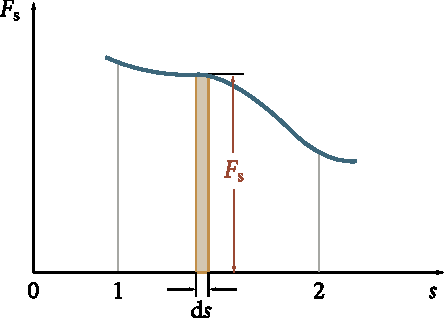
\includegraphics[scale=1]{figures/fig_3_1.pdf}
		\caption[]{}
		\label{fig:3_1}
	\end{center}
	\vspace{-0.7cm}
\end{figure}

Figure~\ref{fig:3_1} is a plot of the projection of the force onto the direction of displacement $F_{\text{s}}$ as a function of the position of the particle on its trajectory (the axis of abscissas has been taken as the $s$-axis, the length of the part of this axis between points $1$ and $2$ equals the total length of the path). Examination of the figure shows that the elementary work $\deriv{A}=F_{\text{s}}\,\deriv{s}$ equals numerically the area of the shaded strip, while the work $A$ over path $1$-$2$ equals numerically the area of the figure confined by the curve $F_{\text{s}}$, the vertical lines from points $1$ and $2$ and the $s$-axis (compare with \fig{1_26}).

Let us use this result to find the work done in the deformation of a spring obeying Hooke's law [see \fig{2_5} and \eqn{2_26}]. We shall begin with stretching of the spring. We shall do this very slowly so that the force $\vec{F}_{\text{ext}}$ which we act on the spring with may be considered equal in magnitude to the elastic force $\vec{F}_{\text{el}}$ all the time. Hence, $\vec{F}_{x,\text{ext}}=-\vec{F}_{x,\text{el}}=kx$, where $x$ is the elongation of the spring (\fig{3_2}). A glance at the figure shows that the work required to cause the elongation $x$ of the spring is
\begin{equation}\label{eq:3_13}
A = \frac{kx^2}{2}.
\end{equation}

\noindent
When the spring is compressed by the amount $x$, work of the same magnitude and sign is done as in stretching by $x$. The projection of the force $\vec{F}_{\text{ext}}$ in this case is negative ($\vec{F}_{\text{ext}}$ is directed to the left, $x$ grows to the right, see \fig{3_2}), and all the $\deriv{x}$'s are also negative. As a result, the product $\vec{F}_{x,\text{ext}}\,\deriv{x}$ is positive.

\begin{figure}[t]
	\begin{center}
		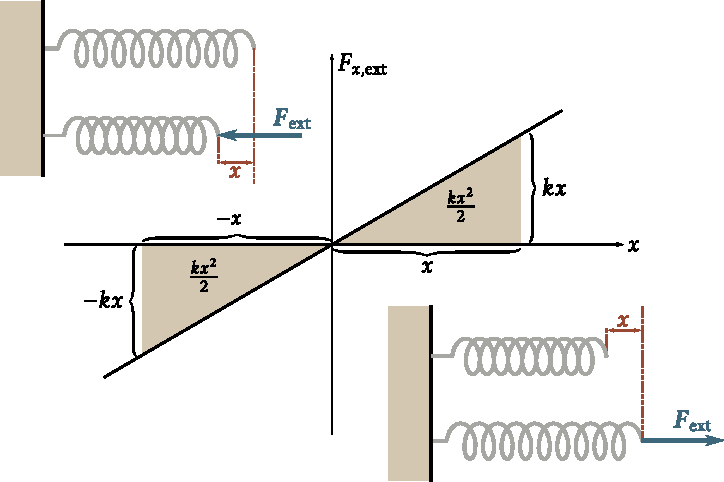
\includegraphics[scale=0.95]{figures/fig_3_2.pdf}
		\caption[]{}
		\label{fig:3_2}
	\end{center}
	\vspace{-0.7cm}
\end{figure}

In a similar way, we can find an expression for the work done upon the elastic stretching or compression of a bar. According to \eqn{2_31}, this work is
\begin{equation}\label{eq:3_14}
A = \frac{1}{2}\frac{ES}{l_0}(\Delta l)^2 = \frac{1}{2}ESl_0\left(\frac{\Delta l}{l_0}\right)^2 = \frac{1}{2}EV\varepsilon^2
\end{equation}

\noindent
where $V=Sl_0$ is the volume of the bar, and $\varepsilon=\Delta l/l_0$ is the relative elongation [see \eqn{2_27}].

Assume that several forces whose resultant is $\vec{F}=\sum_{i}\vec{F}_i$ act simultaneously on a body. It follows from the distributivity of a scalar product of vectors [see \eqn{1_20}] that the work $\deriv{A}$ done by the resultant force over the path $\deriv{s}$ can be represented in the form
\begin{equation}\label{eq:3_15}
\deriv{A} = \left(\sum_{i}\vec{F}_i\right)\deriv{s} = \sum_{i}\vec{F}_i\,\deriv{\vec{s}} = \sum_{i}\deriv{A}_i.
\end{equation}

\noindent
This signifies that the work of the resultant of several forces equals the algebraic sum of the work done by each force separately.

The elementary displacement $\deriv{\vec{s}}$ can be represented as $\vec{v}\deriv{t}$. We can therefore write the expression for the elementary work in the form
\begin{equation}\label{eq:3_16}
\deriv{A} = \vec{F}\vec{v}\,\deriv{t}.
\end{equation}

\noindent
The work done during the interval from $t_1$ to $t_2$ can thus be calculated by the formula
\begin{equation}\label{eq:3_17}
A = \int_{t_1}^{t_2}\vec{F}\,\deriv{t}.
\end{equation}

In accordance with \eqn{1_21}, we have $\vec{F}\,\deriv{\vec{s}}=F\,\deriv{s_F}$, where $\deriv{s_F}$, is the projection of the elementary displacement $\deriv{\vec{s}s}$ onto the direction of the force $\vec{F}$. The formula for work can therefore be written as follows:
\begin{equation}\label{eq:3_18}
\deriv{A} = F\,\deriv{s_F}.
\end{equation}

\begin{figure}[t]
	\begin{center}
		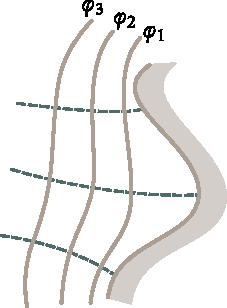
\includegraphics[scale=0.95]{figures/fig_3_3.pdf}
		\caption[]{}
		\label{fig:3_3}
	\end{center}
	\vspace{-0.7cm}
\end{figure}

If the force has a constant magnitude and direction (\fig{3_3}), then the vector $\vec{F}$ in the expression for work may be put outside the integral. The result is
\begin{equation}\label{eq:3_19}
A = \vec{F}\int_{1}^{2}\deriv{\vec{v}} = \vecdot{F}{s} = F s_F
\end{equation}

\noindent
where $\vec{s}$ is the vector of the displacement from point $1$ to point $2$, and $s_F$ is its projection onto the direction of the force.

The work done in unit time is called power. If the work $\deriv{A}$ is done in the time $\deriv{t}$, then the power is
\begin{equation}\label{eq:3_20}
P = \diff{A}{t}.
\end{equation}

\noindent
Taking $\deriv{A}$ as given by \eqn{3_16}, we get the following expression for the power:
\begin{equation}\label{eq:3_21}
P = \vecdot{F}{v}
\end{equation}

\noindent
according to which the power equals the scalar product of the force vector and the vector of the velocity with which the point of application of the force is moving.

\textbf{Units of Work and Power.} The unit of work is the work done by a force equal to unity and acting in the direction of the displacement over a unit distance. Consequently,
\begin{enumerate}[(1)]
	\item in the SI system, the unit of work is the joule (\si{\joule})---the work done by a force of \SI{1}{\newton} over a distance of \SI{1}{\metre};
	\item in the cgs system, the relevant unit is the \si{\erg}---the work done by a force of \SI{1}{\dyne} over a distance of \SI{1}{\centi\metre};
	\item in the mkg(force)s system, the unit is the kilogramme(force)m (\si{\kgf\metre})---the work done by a force of \SI{1}{\kgf} over a distance of \SI{1}{\metre}.
\end{enumerate}

The units of work are related as follows:
\begin{align*}
&\SI{1}{\joule} = \SI{1}{\newton}\times\SI{1}{\metre} = \SI{e5}{\dyne}\times\SI{e2}{\centi\metre} = \SI{e7}{\erg}\\
&\SI{1}{\kgf\metre} = \SI{1}{\kgf}\times\SI{1}{\metre} = \SI{9.81}{\newton}\times\SI{1}{\metre} = \SI{9.81}{\joule}.
\end{align*}

The unit of power is the power at which 1 unit of work is done in unit time. The unit of power in the SI system is the watt (\si{\watt}) equal to one joule per second (\si{\joule\per\second}). The unit of power in the cgs system (\si{\erg\per\second}) has no special name. The relation between the watt and the \si{\erg\per\second} is $\SI{1}{\watt}=\SI{e7}{\erg\per\second}$.

The unit of power in the mkg{force)s system is the (metric) horsepower (\si{\hp}), equal to \SI{75}{\kgf\metre\per\second}, $\SI{1}{\hp}=\SI{736}{\watt}$ (do not confuse this unit with the British or U.S. horsepower equal to \num{550}~ft-lb \si{\per\second} or \SI{746}{\watt}).

A system of prefixes is used, especially in the SI system, to denote multiples and submultiples of units. The names and symbols of these prefixes and the relevant factor by which the basic unit is multiplied are indicated in Table~\ref{table:3_1}.

\begin{table}[!b]
	\renewcommand{\arraystretch}{1.2}
	\caption{Prefixes for Multiples and Submultiples of Units}
	\vspace{-0.6cm}
	\label{table:3_1}
	\begin{center}\resizebox{0.95\linewidth}{!}{
			\begin{tabular}{lcclcc}
				\toprule[1pt]
				& & \textbf{Factor by which} & & & \textbf{Factor by which}\\
				\textbf{Name} & \textbf{Symbol} & \textbf{unit is multiplied} & \textbf{Name} & \textbf{Symbol} & \textbf{unit is multiplied}\\
				\midrule[0.5pt]\midrule[0.5pt]
				Tera & T & \num{e12} & Centi & \si{\centi} & \num{e-2}\\
				Giga & G & \num{e9}  & Milli & \si{\milli} & \num{e-3}\\
				Mega & M & \num{e6}  & Micro & \si{\micro} & \num{e-6}\\
				Kilo & k & \num{e3}  & Nano & \si{\nano} & \num{e-9}\\
				Hecto & h & \num{e2}  & Pico & \si{\pico} & \num{e-12}\\
				Deca & da & \num{e1}  & Femto & \si{\femto} & \num{e-15}\\
				Deci & d & \num{e-1}  & Atto & \si{\atto} & \num{e-18}\\		
				\bottomrule[1pt]
			\end{tabular}
			%	\end{center}
	}\end{center}
\end{table}

For example, the unit of work called the megajoule is equivalent to \num{e6} joules ($\SI{1}{\mega\joule}=\SI{e6}{\joule}$), and the unit of power called the microwatt is equivalent to \num{e-6} watt ($\SI{1}{\micro\watt}=\SI{e-6}{\watt}$}. Similarly, \num{1} micrometer (formerly called the micron) is equivalent to \SI{e-6}{\metre} ($\SI{1}{\micro\metre}=\SI{e-6}{\metre}$), and $\SI{1}{\pico\newton}=\SI{e-12}{\newton}$.

\section{Conservative Forces}\label{sec:3_4}

If a particle is subjected to the action of other bodies at every point of space, the particle is said to be in a field of forces. For example, a particle near the Earth's surface is in the field of gravity forces---at every point of space the force $\vec{P}=m\vec{g}$ acts on it.

\begin{figure}[t]
	\begin{center}
		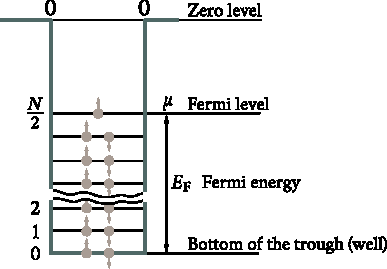
\includegraphics[scale=1]{figures/fig_3_4.pdf}
		\caption[]{}
		\label{fig:3_4}
	\end{center}
	\vspace{-0.7cm}
\end{figure}

Let us consider as a second example the charged particle $e$ in the electric field set up by the fixed point charge $q$ (\fig{3_4}). A feature of this field is that the direction of the force acting on the particle at any point of space passes through a fixed centre (the charge $q$), while the magnitude of the force depends only on the distance to this centre, \ie, $F=F(r)$ [see \eqn{2_23}]. A field of forces with such properties is called a \textbf{central} one.

If at every point of a field the force acting on a particle is identical in magnitude and direction ($\vec{F}=\text{constant}$), the field is called \textbf{homogeneous}.

A field that changes with time is called \textbf{non-stationary}. A field that remains constant with time is called \textbf{stationary}.

For a stationary field, the work done on a particle by the forces of the field may depend only on the initial and final positions of the particle and not depend on the path along which the particle moved. Forces having such a property are called \textbf{conservative}.

\begin{figure}[t]
	\begin{center}
		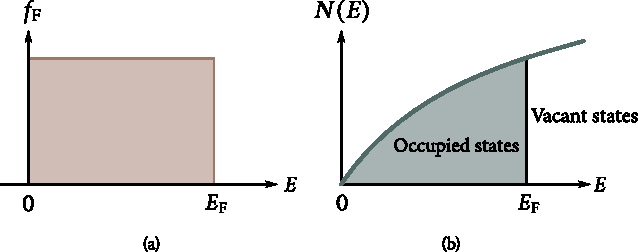
\includegraphics[scale=1]{figures/fig_3_5.pdf}
		\caption[]{}
		\label{fig:3_5}
	\end{center}
\vspace{-0.7cm}
\end{figure}

It follows from the work of conservative forces being independent of the path that the work of such forces along a closed path equals zero. To prove this, let us divide an arbitrary closed path into two parts: path I along which a particle passes from point $1$ to point $2$, and path II along wh1ch the particle passes from point $2$ to point $1$ (\fig{3_5}). We have chosen points $1$ and $2$ arbitrarily. The work along the entire closed path equals the sum of the work done on each of the parts:
\begin{equation}\label{eq:3_22}
A = (A_{12})_{\text{I}} + (A_{21})_{\text{II}}.
\end{equation}

\noindent
It is easy to see that the work $(A_{21})_{\text{II}}$ differs from $(A_{12})_{\text{I}}$ only in its sign. Indeed, reversing of the direction of motion results in $\deriv{\vec{s}}$ being replaced with $-\deriv{\vec{s}}$, and as a consequence the value of the integral $\int\vec{F}\,\deriv{\vec{s}}$ reverses its sign. Thus, \eqn{3_22} can be written in the form
\begin{equation*}
A = (A_{12})_{\text{I}} - (A_{21})_{\text{II}}.
\end{equation*}

\noindent
and since the work does not depend on the path, \ie, $(A_{12})_{\text{I}}=(A_{21})_{\text{II}}$, we arrive at the conclusion that $A=0$.

From the equality to zero of the work over a closed path, it is easy to obtain that the work $A_{12}$ is independent of the path. This can be done by reversing the above reasoning.

Thus, conservative forces can be defined in two ways: (1) as forces whose work does not depend on the path along which a particle passes from one point to another, and (2) as forces whose work along any closed path equals zero.

\begin{figure}[t]
	\begin{minipage}[t]{0.5\linewidth}
		\begin{center}
			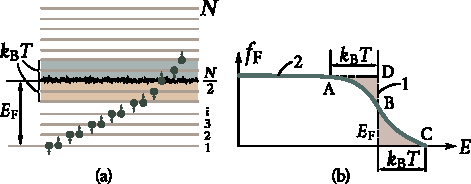
\includegraphics[scale=0.92]{figures/fig_3_6.pdf}
			\caption[]{}
			\label{fig:3_6}
		\end{center}
	\end{minipage}
	\hspace{-0.05cm}
	\begin{minipage}[t]{0.5\linewidth}
		\begin{center}
			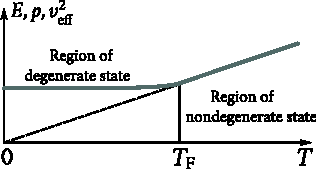
\includegraphics[scale=0.9]{figures/fig_3_7.pdf}
			\caption[]{}
			\label{fig:3_7}
		\end{center}
	\end{minipage}
	\vspace{-0.3cm}
\end{figure}

We shall prove that the force of gravity is conservative. This force at any point has the same magnitude and direction---vertically downward (\fig{3_6}). Therefore, regardless of the path along which the particle moves (for example I or II in the figure), the work $A_{12}$ according to Eq. (3.19) is determined by the expression
\begin{equation*}
A_{12} = m\,(\vecdot{g}{s}_{12}) = mg(s_{12})_{\text{pr. }\vec{g}}.
\end{equation*}

\noindent
Inspection of \fig{3_6} shows that the projection of the vector $\vec{s}_{12}$ onto the direction $\vec{g}$ equals the difference between the heights $h_1-h_2$. Hence, the expression for the work can be written in the form
\begin{equation}\label{eq:3_23}
A_{12} = mg(h_1-h_2).
\end{equation}

\noindent
This expression obviously does not depend on the path. Hence it follows that the force of gravity is conservative. Q.E.D.\footnote{Q.E.D. is an abbreviation of the Latin phrase ``quod erat demonstrandum'', literally meaning ``what was to be shown''.}

It is a simple matter to see that the same result is obtained for any stationary homogeneous field.

The forces acting on a particle in a central field are also conservative. By \eqn{3_18}, the elementary work over the path $\deriv{s}$ (\fig{3_7}) is
\begin{equation*}
\deriv{A} = F(r)\,\deriv{s_F}.
\end{equation*}

\noindent
But the projection of $\deriv{s}$ onto the direction of the force at a given point, \ie, onto the direction of the position vector $\vec{r}$, is $\deriv{r}$---the increment of the distance from the particle to the force centre O, namely, $\deriv{s_F}=\deriv{r}$. Hence, $\deriv{A}=F(r)\,\deriv{r}$, and the work along the entire path is
\begin{equation}\label{eq:3_24}
A_{12} = \int_{r_1}^{r_2} F(r)\,\deriv{r}.
\end{equation}

\noindent
Equation~\eqref{eq:3_24} depends only on the form of the function $F(r)$ and on the values of $r_1$ and $r_2$. It does not depend in any way on the form of the trajectory, whence it follows that the forces are conservative.

For our reader not to form the erroneous idea that any force depending only on the coordinates of a point is conservative, let us consider the following example. Assume that the components of a force are determined by the equations
\begin{equation}\label{eq:3_25}
F_x = ay,\quad F_y = -ax,\quad F_z=0.
\end{equation}

\begin{figure}[t]
	\begin{center}
		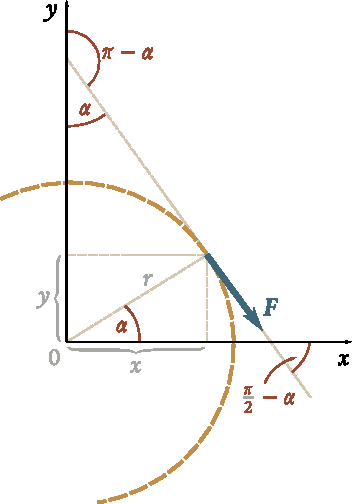
\includegraphics[scale=0.95]{figures/fig_3_8.pdf}
		\caption[]{}
		\label{fig:3_8}
	\end{center}
	\vspace{-0.7cm}
\end{figure}

\noindent
This force has a magnitude equal to $F=ar$, and is directed along a tangent to a circle of radius $r$ (\fig{3_8}). Indeed, as follows from the figure, for a force of such a magnitude and direction, we have
\begin{align*}
F_x &= ar\cos\left(\frac{\pi}{2}-\alpha\right) = ar\sin\alpha = ar\,\frac{y}{r} = ay,\\
F_y &= ar\cos(\pi-\alpha) = ar\cos\alpha = -ar\,\frac{x}{r} = -ax,
\end{align*}

\noindent
which coincides with the values given by Eqs.~\eqref{eq:3_25}. Let us take a closed path in the form of a circle of radius $r$ with its centre at the origin of coordinates. The work of the force along this path evidently equals $F\times 2\pi r=ar\times 2\pi r=2\pi ar^2$ , \ie, does not equal zero. Consequently, the force is not conservative.

Forces of friction are typical non-conservative ones. Since the force of friction $\vec{F}$ and the velocity of a particle $\vec{v}$ are directed oppositely\footnote{Here we have in view friction between a moving body and a stationary (relative to the reference frame) one. The forces of friction may sometimes be positive. This occurs, for instance, when the force of friction is due to the interaction of a given body with another one moving in the same direction, but with a higher velocity.}, then the work of the force of friction on each part of the path is negative:
\begin{equation*}
\deriv{A} = \vec{F}\,\deriv{\vec{s}} = (\vecdot{F}{v})\,\deriv{t} = -Fv\,\deriv{t} = -F\,\deriv{s}<0.
\end{equation*}

\noindent
Therefore, the work along any closed path will also be negative (\ie, other than zero). Hence it follows that the forces of friction are not conservative.

It must be noted that a field of conservative forces is a particular case of a potential force field. A field of forces is called \textbf{potential} if it can be described with the aid of the function $V(x,y,z,t)$, whose gradient [see the following section, \eqn{3_31}] determines the force at each point of the field: $\vec{F}=\nabla V$ [compare with \eqn{3_32}]. The function $V$ is called the \textbf{potential function} or the \textbf{potential}.

When a potential does not depend explicitly on the time, \ie, $V=V(x,y,z)$, the potential field is stationary, and its forces are conservative. In this case
\begin{equation*}
V(x,y,z) = -E_{\text{p}}(x,y,z)
\end{equation*}

\noindent
where $E_{\text{p}}(x,y,z)$ is the potential energy of a particle (see the following section).

For a non-stationary force field described by the potential $V(x,y,z,t)$, the potential and conservative forces cannot be considered identical.

\section{Potential Energy in an External Force Field}\label{sec:3_5}

Let us consider the case when the work of field forces does not depend on the path, but depends only on the initial and final positions of a particle in the field. A value of a certain function $E_{\text{p}}(x,y,z)$ can be assigned to each point of the field such that the difference between the values of this function at points $1$ and $2$ will determine the work of the forces when the particle passes from the first point to the second one:
\begin{equation}\label{eq:3_26}
A_{12} = E_{\text{p},1} - E_{\text{p},2}.
\end{equation}

We can assign this function as follows. We take an arbitrary value of the function equal to $E_{\text{p},0}$ , for an initial point $0$. We assign the value
\begin{equation}\label{eq:3_27}
E_{\text{p}}(P) = E_{\text{p},0} + A_{\text{p},0}
\end{equation}

\noindent
to any other point $P$. Here $A_{\text{p},0}$ is the work done on a particle by the conservative forces when it is moved from point $P$ to point $0$. Since the work is independent of the path, the value of $E_{\text{p}}(P)$ determined in this way will be unambiguous. It must be noted that the function $E_{\text{p}}(P)$ has the dimension of work (or energy).

In accordance with \eqn{3_27}, the values of the function at points $1$ and $2$ are
\begin{equation*}
E_{\text{p},1} = E_{\text{p},0} + A_{10},\quad E_{\text{p},2} = E_{\text{p},0} + A_{20}.
\end{equation*}

\noindent
Let us form the difference between these values and take into account that $A_{20}=-A_{02}$ (see the preceding section). As a result, we get
\begin{equation*}
E_{\text{p},1} - E_{\text{p},2} = A_{10} - A_{20} = A_{10} + A_{02}.
\end{equation*}

\noindent
The sum $A_{10}+A_{02}$ gives the work done by the forces of the field when the particle moves from point $1$ to point $2$ along a trajectory passing through point $0$. However, the work done to move the particle from point $1$ to point $2$ along any other trajectory (including one not passing through point $0$) will be the same. Hence, the sum $A_{10}+A_{02}$ can be written simply in the form $A_{12}$. As a result, we get \eqn{3_26}.

We can thus use the function $E_{\text{p}}$ to determine the work done on a particle by conservative forces along any path beginning at arbitrary point $1$ and terminating at arbitrary point $2$.

Assume that only conservative forces act on the particle. Consequently, the work done on the particle along path $1$-$2$ can be represented in the form of \eqn{3_26}. According to \eqn{3_11}, this work produces an increment of the kinetic energy of the particle. We thus arrive at the equation
\begin{equation*}
E_{\text{k},2} - E_{\text{k},1} = E_{\text{p},1} - E_{\text{p},2}
\end{equation*}

\noindent
whence it follows that
\begin{equation*}
E_{\text{k},2} + E_{\text{p},2} = E_{\text{k},1} + E_{\text{p},1}
\end{equation*}

\noindent
The result obtained signifies that the quantity
\begin{equation}\label{eq:3_28}
E = E_{\text{k}} + E_{\text{p}}
\end{equation}

\noindent
for a particle in the field of conservative forces remains constant, \ie, is an integral of motion.

It follows from \eqn{3_28} that $E_{\text{p}}$ is an addend in the motion integral having the dimension of energy. In this connection, the function $E_{\text{p}}(x,y,z)$ is called the \textbf{potential energy} of a particle in an external force field. The quantity $E$ equal to the sum of the kinetic and potential energies is called the \textbf{total mechanical energy} of the particle.

According to \eqn{3_26}, the work done on a particle by conservative forces equals the decrement of the potential energy of the particle.

We can say in a different way that work is done at the expense of the store of potential energy. We can see from \eqn{3_27} that the potential energy is determined with an accuracy to a certain unknown additive constant $E_{\text{p},0}$. This circumstance is of no significance, however, because all physical relations contain either the difference between the values of $E_{\text{p}}$ for two positions of a body, or the derivative of the function $E_{\text{p}}$ with respect to the coordinates. In practice, the potential energy of a body at a certain position is considered to equal zero, and the energy at other positions is taken with respect to this energy.

Knowing the form of the function $E_{\text{p}}(x,y,z)$, we can find the force acting on a particle at every point of a field. Let us consider the displacement of a particle parallel to the $x$-axis by the amount $\deriv{x}$. This displacement is attended by work being done on the particle that is $\deriv{A}=\vec{F}\,\deriv{\vec{s}}=F_x\,\deriv{x}$ (the displacement components $\deriv{y}$ and $\deriv{z}$ equal zero). According to \eqn{3_26}, the same work can be represented as the decrement of the potential energy: $\deriv{A}=-\deriv{E_{\text{p}}}$. Equating the two expressions for the work, we obtain
\begin{equation*}
F_x\,\deriv{x} = -\deriv{E_{\text{p}}}
\end{equation*}

\noindent
whence
\begin{equation*}
F_x = -\diff{E_{\text{p}}}{x}\, (y=\text{constant},\, z=\text{constant}).
\end{equation*}

\noindent
The expression in the right-hand side is the derivative of the function $E_{\text{p}}(x,y,z)$ calculated on the assumption that the variables $y$ and $z$ remain constant, and only the variable $x$ changes. Such derivatives are called partial ones and are denoted, unlike derivative functions of one variable, by the symbol $\diffinpartial{E_{\text{p}}}{x}$. Consequently, the component of the force along the $x$-axis equals the partial derivative of the potential energy with respect to the variable $x$ taken with the opposite sign: $F_x=-\diffinpartial{E_{\text{p}}}{x}$. Similar expressions are obtained for the components of the force along the $y$- and $z$-axes. Thus,
\begin{equation}\label{eq:3_29}
F_x = -\diffpartial{E_{\text{p}}}{x},\quad F_y = -\diffpartial{E_{\text{p}}}{y},\quad F_z = -\diffpartial{E_{\text{p}}}{z}.
\end{equation}

Knowing its components, we can find the force vector:
\begin{equation}\label{eq:3_30}
\vec{F} = F_x\vecuni{x} + F_y\vecuni{y} + F_z\vecuni{z} = 
-\diffpartial{E_{\text{p}}}{x}\vecuni{x} - \diffpartial{E_{\text{p}}}{y}\vecuni{y} -\diffpartial{E_{\text{p}}}{z}\vecuni{z}.
\end{equation}

A vector having the components $\diffinpartial{\varphi}{x}$,  $\diffinpartial{\varphi}{y}$, $\diffinpartial{\varphi}{z}$, where $\varphi$ is a scalar function of the coordinates $x,y,z$, is called the gradient of the function $\varphi$ and is designated by the symbol grad $\varphi$ or $\nabla\varphi$ ($\nabla$ stands for the \textbf{nabla operator}). It follows from the definition of the gradient that
\begin{equation}\label{eq:3_31}
\nabla\varphi = \diffpartial{\varphi}{x}\vecuni{x} + \diffpartial{\varphi}{y}\vecuni{y} + \diffpartial{\varphi}{z}\vecuni{z}.
\end{equation}

A comparison of Eqs.~\eqref{eq:3_30} and~\eqref{eq:3_31} shows that the conservative force equals the gradient of the potential energy taken with the opposite sign:
\begin{equation}\label{eq:3_32}
\vec{F} = -\nabla E_{\text{p}}.
\end{equation}

Assume that a particle which the force~\eqref{eq:3_32} acts on moves over the distance $\deriv{\vec{s}}$ having the components $\deriv{x}$, $\deriv{y}$, $\deriv{z}$. The force does the work
\begin{equation*}
\deriv{A} = \vec{F}\,\deriv{\vec{s}} = -\nabla E_{\text{p}}\,\deriv{\vec{s}} = - \left(\diffpartial{E_{\text{p}}}{x}\,\deriv{x} + \diffpartial{E_{\text{p}}}{y}\,\deriv{y} +  \diffpartial{E_{\text{p}}}{z}\,\deriv{z}\right).
\end{equation*}

\noindent
Taking into account that $\deriv{A}=-\deriv{E_{\text{p}}}$, we get the following expression for the increment of the function $E_{\text{p}}$:
\begin{equation}\label{eq:3_33}
\deriv{E_{\text{p}}} = \diffpartial{E_{\text{p}}}{x}\,\deriv{x} + \diffpartial{E_{\text{p}}}{y}\,\deriv{y} +  \diffpartial{E_{\text{p}}}{z}\,\deriv{z}.
\end{equation}

\noindent
An expression such as \eqn{3_33} is called the total differential of the relevant function.

The concept of the total differential plays a great part in physics. For this reason, we shall devote a few lines to it. The \textbf{total differential} of the single-valued function $f(x,y,z)$ is defined as the increment which this function receives in transition from a point with the coordinates $x,y,z$ to a neighbouring point with the coordinates $x+\deriv{x}, y+\deriv{y}, z+\deriv{z}$. By definition, this increment equals
\begin{equation*}
\deriv{f}(x,y,z) = f(x+\deriv{x}, y+\deriv{y}, z+\deriv{z}) - f(x,y,z) 
\end{equation*}

\noindent
and, consequently, is determined only by the values of the function at the initial and final points. Hence, it cannot depend on the path along which the transition occurs. Let us take the broken line consisting of the segments $\deriv{x}, \deriv{y}, \deriv{z}$ as such a path (\fig{3_9}). On the segment $\deriv{x}v$, the function $f(x,y,z)$ behaves like a function of one variable $x$, and receives the increment $(\diffinpartial{f}{x})\,\deriv{x}$. Similarly, on the segments $\deriv{y}$ and $\deriv{z}$, the function receives the increments $(\diffinpartial{f}{y})\,\deriv{y}$ and $(\diffinpartial{f}{z})\,\deriv{z}$. The total increment of the function when passing from the initial point to the final one thus equals
\begin{equation}\label{eq:3_34}
\deriv{f}(x,y,z)  = \diffpartial{f}{x}\,\deriv{x} + \diffpartial{f}{y}\,\deriv{y} +  \diffpartial{f}{z}\,\deriv{z}.
\end{equation}

\noindent
We have arrived at the expression for the total differential [compare with \eqn{3_33}].

\begin{figure}[t]
	\begin{center}
		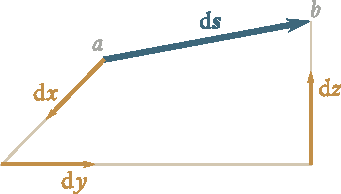
\includegraphics[scale=0.95]{figures/fig_3_9.pdf}
		\caption[]{}
		\label{fig:3_9}
	\end{center}
	\vspace{-0.7cm}
\end{figure}

Not any expression of the kind
\begin{equation*}
P(x,y,z)\deriv{x} + Q(x,y,z)\deriv{y} + R(x,y,z)\deriv{z}
\end{equation*}

\noindent
is a total differential of a certain function $f(x,y,z)$. Particularly, the expression for the work done by the force whose projections are given by Eqs.~\eqref{eq:3_25}
\begin{equation}\label{eq:3_35}
\deriv{A} = ay\,\deriv{x} - ax\,\deriv{y}
\end{equation}

\noindent
is not a total differential because there is no such function $E_{\text{p}}$ for which $-\diffinpartial{E_{\text{p}}}{x}=ay$, and $-\diffinpartial{E_{\text{p}}}{y}=-ax$ [see Eqs.~\eqref{eq:3_25}]. Correspondingly, there is no function $E_{\text{p}}$ whose decrement would determine the work~\eqref{eq:3_35}.

It follows from the above that only forces complying with the condition~\eqref{eq:3_32} can be conservative, \ie, such forces whose components along the coordinate axes equal the derivatives of a certain function $E_{\text{p}}(x,y,z)$ with respect to the relevant coordinates taken with the opposite sign. This function is the potential energy of a particle.

The concrete form of the function $E_{\text{p}}(x,y,z)$ depends on the nature of the force field. Let us find as an example the potential energy of a particle in a field of forces of gravity. According to \eqn{3_23}, the work done on a particle by the forces of this field is
\begin{equation*}
A_{12} = mg(h_1-h_2).
\end{equation*}

\noindent
On the other hand, according to \eqn{3_26},
\begin{equation*}
A_{12} = E_{\text{p},1} - E_{\text{p},2}.
\end{equation*}

\noindent
Comparing these two expressions for the work, we arrive at the conclusion that the potential energy of a particle in a field of gravity forces is determined by the expression
\begin{equation}\label{eq:3_36}
E_{\text{p}} = mgh
\end{equation}

\noindent
where $h$ is measured from an arbitrary level.

The zero of potential energy may be chosen arbitrarily. Therefore, $E_{\text{p}}$ may have negative values. If we take the potential energy of a particle on the Earth's surface as zero, for example, then the potential energy of a particle lying on the bottom of a pit with a depth of $h'$ will be $E_{\text{p}}=-mgh'$ (\fig{3_10}). It must be noted that the kinetic energy cannot be negative.

\begin{figure}[t]
	\begin{center}
		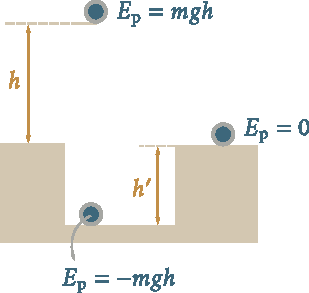
\includegraphics[scale=1]{figures/fig_3_10.pdf}
		\caption[]{}
		\label{fig:3_10}
	\end{center}
	\vspace{-0.7cm}
\end{figure}

Assume that the non-conservative force $\vec{F}^*$ acts on a particle in addition to conservative forces. Hence, when the particle is moved from point $1$ to point $2$, the work done on it will be
\begin{equation*}
A_{12} = \int_{1}^{2} \vec{F}\,\deriv{\vec{s}} + \int_{1}^{2} \vec{F}^*\,\deriv{\vec{s}} = A_{\text{cons}} + A_{12}^*
\end{equation*}

\noindent
where $A_{12}^*$ is the work of the non-conservative force. The work of the conservative forces $A_{\text{cons}}$ can be represented as $E_{\text{p},1}-E_{\text{p},2}$. As a result, we find that
\begin{equation*}
A_{12} = E_{\text{p},1} - E_{\text{p},2} + A_{12}^*
\end{equation*}

\noindent
The total work of all the forces applied to the particle produces an increment of its kinetic energy [see \eqn{3_11}]. Consequently,
\begin{equation*}
E_{\text{k},2} - E_{\text{p},1} = E_{\text{p},1} - E_{\text{p},2} + A_{12}^*
\end{equation*}

\noindent
whence, taking into consideration that $E_{\text{k}}+E_{\text{p}}=E$, we get
\begin{equation}\label{eq:3_37}
E_2 - E_1 = A_{12}^*.
\end{equation}

\noindent
The result obtained signifies that the work of non-conservative forces is spent on an increment of the total mechanical energy of a particle.

If the kinetic energy of a particle is the same in its final and initial  positions (in particular, it equals zero), then the work of the non-conservative forces produces an increment of the potential energy of the particle:
\begin{equation}\label{eq:3_38}
A_{12}^* = E_{\text{p},2} - E_{\text{p},1}
\end{equation}

\noindent
($E_{\text{k},2}=E_{\text{k},1}$). This relation is useful when finding the difference between the values of the potential energy.

Let us consider a system consisting of $N$ particles in the field of conservative forces when the particles do not interact with one another. Each of the particles has the kinetic energy $E_{\text{k},i}=m_iv_i^2/2$ ($i$ is the number of the particle) and the potential energy $E_{\text{p},i}=E_{\text{p},i}(x_i,y_i,z_i)$. Considering the $i$-th particle independently of the other particles, we can find that
\begin{equation*}
E_i = E_{\text{k},i} + E_{\text{p},i} = \text{constant}_i
\end{equation*}

\noindent
Summing these equations for all the particles, we arrive at the relation
\begin{equation}\label{eq:3_39}
E = \sum_{i=1}^{N}E_i = \sum_{i=1}^{N}E_{\text{k},i} + \sum_{i=1}^{N}E_{\text{p},i} = \text{constant}. 
\end{equation}

\noindent
This relation points to the additivity of the total mechanical energy for the system being considered.

According to \eqn{3_39}, \textit{the total mechanical energy of a system of non-interacting particles on which only conservative forces act remains constant}. This statement expresses the law of energy conservation for the above mechanical system.

If non-conservative forces $\vec{F}^*$ act on particles in addition to conservative forces, the total energy of the system does not remain constant, and
\begin{equation}\label{eq:3_40}
E_2 - E_1 = \sum_{i=1}^{N}(A_{12}^*)_i 
\end{equation}

\noindent
where $(A_{12}^*)_i$ is the work done by the non-conservative force applied to the $i$-th particle when it moves from its initial position to its final one.

We established at the end of the preceding section that the work of friction forces is always negative. Therefore, when such forces are present in a system, the total mechanical energy of the system diminishes (dissipates), transforming into non-mechanical forms of energy (for example, into the internal energy of bodies, or, as is customarily said, into heat). This process is called the \textbf{dissipation} of energy. Forces leading to the dissipation of energy are called \textbf{dissipative}. Thus, friction forces are dissipative. In general, forces that always act oppositely to the velocities of particles and therefore cause their retardation are called dissipative.

We shall note that non-conservative forces are not necessarily dissipative ones.

\section{Potential Energy of Interaction}\label{sec:3_6}

Up to now, we treated systems of non-interacting particles. Now we shall pass over to the consideration of a system of two particles interacting with each other. Let $\vec{F}_{12}$ be the force with which the second particle acts on the first one, and $\vec{F}_{21}$ be the force with which the first particle acts on the second one. In accordance with Newton's third law, $\vec{F}_{12}=-\vec{F}_{21}$.

%\begin{figure}[t]
%	\begin{center}
%		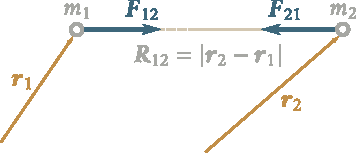
\includegraphics[scale=1]{figures/fig_3_11.pdf}
%		\caption[]{}
%		\label{fig:3_11}
%	\end{center}
%%	\vspace{-0.7cm}
%\end{figure}

Let us introduce the vector $\vec{R}_{12}=\vec{r}_2-\vec{r}_1$ , where $\vec{r}_1$ and $\vec{r}_2$ are the position vectors of the particles (\fig{3_11}). The distance between the particles equals the magnitude of this vector. Assume that the magnitudes of the forces $\vec{F}_{12}$ and $\vec{F}_{21}$ depend only on the distance $\vec{R}{12}$ between the particles, and that the forces are directed along the straight line connecting the particles. We know that this holds for forces of gravitational and Coulomb interactions [see Eqs.~\eqref{eq:2_18} and~\eqref{eq:2_23}].

With these assumptions, the forces $\vec{F}_{12}$ and $\vec{F}_{21}$ can be represented in the form
\vspace{-12pt}
\begin{equation}\label{eq:3_41}
\vec{F}_{12} = -\vec{F}_{21} = f(R_{12})\vecuni{12}
\end{equation}

\noindent
where $\vecuni{12}$ is the unit vector of $\vec{R}_{12}$ (\fig{3_12}), and $f(R_{12})$ is a certain function of $R_{12}$ that is positive when the particles attract each other and negative when they repel each other.

Considering our system to be closed (there are no external forces), let us write the equations of motion for our two particles:
\begin{equation*}
m_1\dot{\vec{v}}_1 = \vec{F}_{12},\quad m_2\dot{\vec{v}}_2 = \vec{F}_{21}
\end{equation*}

\noindent
Let us multiply the first equation by $\deriv{\vec{r}_1}=\vec{v}_1\,\deriv{t}$, the second by $\deriv{\vec{r}_2}=\vec{v}_2\,\deriv{t}$, and add the resulting equations\footnote{Here it is expedient to use the symbol $\deriv{r}$ for the displacement instead of $\deriv{\vec{s}}$.}. We get
\begin{equation}\label{eq:3_42}
m_1\vec{v}_1\dot{\vec{v}}_1\,\deriv{t} + m_2\vec{v}_2\dot{\vec{v}}_2\,\deriv{t} = \vec{F}_{12}\,\deriv{\vec{r}_1} + \vec{F}_{21}\,\deriv{\vec{r}_2}.
\end{equation}

\begin{figure}[t]
	\begin{minipage}[t]{0.5\linewidth}
		\begin{center}
			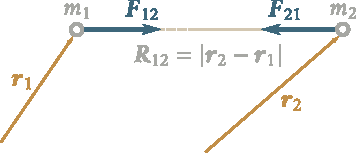
\includegraphics[scale=0.89]{figures/fig_3_11.pdf}
			\caption[]{}
			\label{fig:3_11}
		\end{center}
	\end{minipage}
	\hspace{-0.05cm}
	\begin{minipage}[t]{0.5\linewidth}
		\begin{center}
			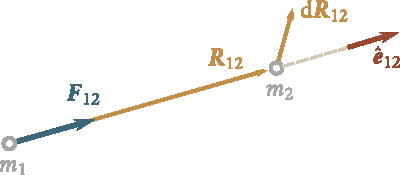
\includegraphics[scale=0.89]{figures/fig_3_12.pdf}
			\caption[]{}
			\label{fig:3_12}
		\end{center}
	\end{minipage}
	%	\vspace{-0.7cm}
\end{figure}

\noindent
The left-hand side of this equation is the increment of the kinetic energy of the system during the time $\deriv{t}$ [see \eqn{3_3}], and the right-hand side is the work of the internal forces during the same time. Taking into account that $\vec{F}_{21}=-\vec{F}_{12}$, we can write the right-hand side as follows:
\begin{equation}\label{eq:3_43}
\deriv{A}_{\text{int}} = \vec{F}_{12}\,\deriv{\vec{r}_1} + \vec{F}_{21}\,\deriv{\vec{r}_2} = -\vec{F}_{12}\,\deriv{(\vec{r}_2-\vec{r}_1)} = -\vec{F}_{12}\,\deriv{\vec{R}_{12}}.
\end{equation}

\noindent
Introducing \eqn{3_41} for $\vec{F}_{12}$ into the above equation, we get
\begin{equation*}
\deriv{A}_{\text{int}} = - f(R_{12}) \vecuni{12} \, \deriv{\vec{R}_{12}}.
\end{equation*}

\noindent
Examination of \fig{3_12} shows that the scalar product $\vecuni{12}\,\deriv{\vec{R}_{12}}$ equals $\deriv{R_{12}}$---the increment of the distance between the particles. Thus,
\begin{equation}\label{eq:3_44}
\deriv{A}_{\text{int}} = - f(R_{12})\,\deriv{R_{12}}.
\end{equation}

%\begin{figure}[t]
%	\begin{center}
%		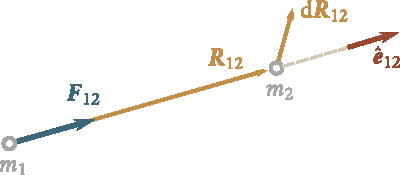
\includegraphics[scale=1]{figures/fig_3_12.pdf}
%		\caption[]{}
%		\label{fig:3_12}
%	\end{center}
%%	\vspace{-0.7cm}
%\end{figure}

The expression $f(R_{12})\,\deriv{R_{12}}$ can be considered as the increment of a certain function of $R_{12}$. Designating this function $E_{\text{p}}(R_{12})$, we arrive at the equation
\begin{equation}\label{eq:3_45}
f(R_{12})\,\deriv{R_{12}} = \deriv{E_{\text{p}}(R_{12})}.
\end{equation}

\noindent
Consequently,
\begin{equation}\label{eq:3_46}
\deriv{A}_{\text{int}} = \deriv{E_{\text{p}}}.
\end{equation}

With a view to everything said above, \eqn{3_42} can be written in the form $\deriv{E_{\text{k}}}=-\deriv{E_{\text{p}}}$, or
\begin{equation}\label{eq:3_47}
\deriv{E} = \deriv{(E_{\text{k}}+E_{\text{p}})} = 0
\end{equation}

\noindent
whence it follows that the quantity $E=E_{\text{k}}+E_{\text{p}}$ for the closed system being considered remains unchanged. The function $E_{\text{p}}(R_{12})$ is the potential energy of interaction. It depends on the distance between the particles.

Let the particles move from their positions spaced $R_{12}^{(a)}$ apart to new positions spaced $R_{12}^{(b)}$ apart. In accordance with \eqn{3_46}, the internal forces do the following work on the particles:
\begin{equation}\label{eq:3_48}
A_{\text{ab, int}} = - \int_{a}^{b} \deriv{E_{\text{p}}} = E_{\text{p}}[R_{12}^{(a)}] - E_{\text{p}}[R_{12}^{(b)}].
\end{equation}

\noindent
It follows from \eqn{3_48} that the work of the forces~\eqref{eq:3_41} does not depend on the paths of the particles and is determined only by the initial and final distances between them (the initial and final configurations of the system). Forces of interaction of the form given by \eqn{3_41} are thus conservative.

If both particles move, the total energy of the system is
\begin{equation}\label{eq:3_49}
E = \frac{m_1v_1^2}{2} + \frac{m_2v_2^2}{2} + E_{\text{p,ia}}(R_{12})
\end{equation}

\noindent
where $E_{\text{p,ia}}(R_{12})$ is the potential energy of interaction.

Assume that particle $1$ is fixed at a certain point which we shall take as the origin of coordinates ($\vec{r}_1=0$). As a result, this particle will lose its ability to move, so that the kinetic energy will consist only of the single addend $m_2v_2^2/2$. The potential energy will be a function only of $\vec{r}_2$. Therefore, \eqn{3_49} becomes
\begin{equation}\label{eq:3_50}
E = \frac{m_2v_2^2}{2} + E_{\text{p,ia}}(r_2).
\end{equation}

\noindent
If we consider the system consisting of only the single particle $2$, then the function $E_{\text{p,ia}}$ will play the part of the potential energy of particle $2$ in the field of the forces set up by particle $1$. In essence, however, this function is the potential energy of interaction of particles $1$ and $2$. In general, the potential energy in an external field of forces is essentially the energy of interaction between the bodies of the system and those producing a force field that is external relative to the system.

Let us again turn to a system of two interacting free (``unfixed'') particles. If the external force $\vec{F}_1^*$ acts on the first particle in addition to the internal force, and the force $\vec{F}_2^*$ on the second particle, then the addends $\vec{F}_1^*\,\deriv{\vec{r}_1^*}$ and $\vec{F}_2^*\,\deriv{\vec{r}_2^*}$ will appear in the right-hand side of \eqn{3_42}, and their sum will give the work of the external forces $\deriv{A_{\text{ext}}}$. Equation~\eqref{eq:3_47} will correspondingly become
\begin{equation}\label{eq:3_51}
\deriv{(E_{\text{k}}+E_{\text{p,ia}})} = \deriv{A_{\text{ext}}}.
\end{equation}

When the total kinetic energy of the particles remains constant (for example, equals zero), \eqn{3_51} becomes
\begin{equation}\label{eq:3_52}
\deriv{E_{\text{p,ia}}} = \deriv{A_{\text{ext}}}
\end{equation}

\noindent
(here $\deriv{E_{\text{k}}}=0$). Integration of this equation from configuration $a$ to configuration $b$ yields
\begin{equation}\label{eq:3_53}
E_{\text{p,ia}}[R_{12}^{(b)}] - E_{\text{p,ia}}[R_{12}^{(a)}] = \deriv{A_{\text{ab,ext}}}
\end{equation}

\noindent
($E_{\text{k},b}=E_{\text{k},a}$) [compare with \eqn{3_38}].

Let us extend the results obtained to a system of three interacting particles. In this case, the work of the internal forces is
\begin{equation}\label{eq:3_54}
\deriv{A_{\text{int}}} = (\vec{F}_{12} + \vec{F}_{13})\,\deriv{\vec{r}_1} + (\vec{F}_{21} + \vec{F}_{23})\,\deriv{\vec{r}_2} + (\vec{F}_{31} + \vec{F}_{32})\,\deriv{\vec{r}_3}.
\end{equation}

\noindent
Taking into account that $\vec{F}_{ik}=-\vec{F}_{ki}$ we can write \eqn{3_54} in the form
\begin{align}
\deriv{A_{\text{int}}} &= - \vec{F}_{12}\,\deriv{(\vec{r}_2-\vec{r}_1)} - \vec{F}_{13}\,\deriv{(\vec{r}_3-\vec{r}_1)} - \vec{F}_{23}\,\deriv{(\vec{r}_3-\vec{r}_2)}\nonumber\\
&= - \vec{F}_{12}\,\deriv{\vec{R}_{12}} - \vec{F}_{13}\,\deriv{\vec{R}_{13}} - \vec{F}_{23}\,\deriv{\vec{R}_{23}}\label{eq:3_55}
\end{align}

\noindent
where $\vec{R}_{ik}=\vec{r}_k-\vec{r}_i$.

Let us assume that the internal forces can be represented in the form $\vec{F}_{ik}=f_{ik}(R_{ik})\vecuni{ik}$ [compare with \eqn{3_41}]. Hence,
\begin{equation*}
\deriv{A_{\text{int}}} = - f_{12}(R_{12})\vecuni{12}\,\deriv{\vec{R}_{12}} - f_{13}(R_{13})\vecuni{13}\,\deriv{\vec{R}_{13}} - f_{23}(R_{23})\vecuni{23}\,\deriv{\vec{R}_{23}}. \end{equation*}

\noindent
Each of the products $\vecuni{ik}\,\deriv{R_{ik}}$ equals the increment of the distance between the corresponding particles $\deriv{R_{ik}}$. Consequently,
\begin{align}
\deriv{A_{\text{int}}} &= - f_{12}(R_{12})\,\deriv{R_{12}} - f_{13}(R_{13})\,\deriv{R_{13}} - f_{23}(R_{23})\,\deriv{R_{23}}\nonumber\\
&= - \deriv{[E_{\text{p},12}(R_{12}) + E_{\text{p},13}(R_{13}) + E_{\text{p},23}(R_{23})]} = - \deriv{E_{\text{p,ia}}}.\label{eq:3_56}
\end{align}

\noindent
Here
\begin{equation}\label{eq:3_57}
E_{\text{p,ia}} = E_{\text{p},12}(R_{12}) + E_{\text{p},13}(R_{13}) + E_{\text{p},23}(R_{23})
\end{equation}

\noindent
is the \textbf{potential energy of interaction of the system}. It consists of the energies of interaction of the particles taken in pairs.

Equating $\deriv{E_{\text{k}}}$ to the sum of the work $\deriv{A_{\text{int}}}=-\deriv{E_{\text{p,ia}}}$ and $\deriv{A_{\text{ext}}}$ we arrive at \eqn{3_51} in which by $E_{\text{p,ia}}$ we must understand \eqn{3_57}.

The result obtained is easily generalized for a system with any number of particles. For a system of $N$ interacting particles, the potential energy of interaction consists of the energies of interaction of the particles taken in pairs:
\begin{multline}\label{eq:3_58}
E_{\text{p,ia}} = E_{\text{p},12}(R_{12}) + E_{\text{p},13}(R_{13}) + \ldots + E_{\text{p},1N}(R_{1N})\\
+ E_{\text{p},23}(R_{23}) + E_{\text{p},2N}(R_{2N}) + \ldots + E_{\text{p},N-1,N}(R_{N-1,N}).
\end{multline}

\noindent
This sum can be written as follows:
\begin{equation}\label{eq:3_59}
E_{\text{p,ia}} = \sum_{i<k} E_{\text{p},ik}(R_{ik})
\end{equation}

\noindent
[note that in \eqn{3_58} the first subscript of each addend has a value smaller than the second one]. In connection with the fact that $E_{\text{p},ik}(R_{ik})=E_{\text{p},ki}(R_{ki})$, the energy of interaction can also be represented in the form
\begin{equation}\label{eq:3_60}
E_{\text{p,ia}} = \frac{1}{2}\,\sum_{i\neq k} E_{\text{p},ik}(R_{ik}).
\end{equation}

\noindent
In the sums~\eqref{eq:3_59} and~\eqref{eq:3_60}, the subscripts $i$ and $k$ take on values from $1$ to $N$ with observance of the condition that $i<k$ or $i\neq k$.

Assume that a system consists of four particles, and that the first particle interacts only with the second one and the third particle only with the fourth one. The total energy of this system will be
\begin{align}
E &= E_{\text{k},1} + E_{\text{k},2} + E_{\text{k},3} + E_{\text{k},4} + E_{\text{k},12} + E_{\text{k},34}\nonumber\\
&= (E_{\text{k},1} + E_{\text{k},2} + E_{\text{k},12}) + (E_{\text{k},3} + E_{\text{k},4} + E_{\text{k},34}) = E' + E''. \label{eq:3_61}
\end{align}

\noindent
Here $E'$ is the total energy of the subsystem formed by particles $1$ and $2$, and $E''$ is the total energy of the subsystem formed by particles $3$ and $4$. In accordance with our assumption, there is no interaction between the subsystems. Equation~\eqref{eq:3_61} proves the additivity of energy (see the third paragraph of Sec.~\ref{sec:3_1}).

In conclusion, let us find the form of the function $E_{\text{p,ia}}$ for the case when the force of interaction is inversely proportional to the square of the distance between the particles:
\begin{equation}\label{eq:3_62}
f(R_{12}) = \frac{\alpha}{R_{12}^2}
\end{equation}

\noindent
($\alpha$ is a constant). We remind our reader that for attraction between the particles $\alpha>0$, and for repulsion between them $\alpha<0$ [see the text following \eqn{3_41}].

In accordance with \eqn{3_45}
\begin{equation*}
\deriv{E_{\text{p,ia}}} = f(R_{12})\,\deriv{R_{12}} = \frac{\alpha}{R_{12}^2}\,\deriv{R_{12}}.
\end{equation*}

\noindent
Integration yields
\begin{equation}\label{eq:3_63}
E_{\text{p,ia}} = - \frac{\alpha}{R_{12}} + \text{constant}.
\end{equation}

Like the potential energy in an external field of forces, the potential energy of interaction is determined with an accuracy up to an arbitrary additive constant. It is usually assumed that when $R_{12}=\infty$, the potential energy becomes equal to zero [at such a distance the force \eqn{3_62} becomes equal to zero---the interaction between the particles vanishes]. Hence, the additive constant in \eqn{3_63} vanishes, and the expression for the potential energy of interaction acquires the form
\begin{equation}\label{eq:3_64}
E_{\text{p,ia}} = - \frac{\alpha}{R_{12}}.
\end{equation}

In accordance with \eqn{3_53}, the following work must be done to move the particles away from each other from the distance $R_{12}$ to infinity without changing their velocities:
\begin{equation*}
A_{\text{ext}} = E_{\text{p,ia}}(\infty) - E_{\text{p,ia}}(R_{12}).
\end{equation*}

\noindent
Introduction of the corresponding values of the function \eqn{3_64} leads to the expression
\begin{equation}\label{eq:3_65}
A_{\text{ext}} = 0 - \left(-\frac{\alpha}{R_{12}}\right) = \frac{\alpha}{R_{12}}.
\end{equation}

When the particles are attracted to each other, we have $\alpha>0$; accordingly, positive work must be done to move the particles away from each other.

Upon repulsion of the particles from each other, $\alpha<0$, and the work~\eqref{eq:3_65} is negative. This work has to be done to prevent the particles that are repelling each other from increasing their velocity.

%\vspace{-12pt}

\section{Law of Conservation of Energy}\label{sec:3_7}

Let us combine the results obtained in the preceding sections. We shall consider a system consisting of $N$ particles of masses $m_1, m_2, \ldots, m_N$. Assume that the particles interact with one another with the forces $\vec{F}_{ik}$, whose magnitudes depend only on the distance $R_{ik}$ between the particles. We established in the preceding section that such forces are conservative. This signifies that the work done by these forces on the particles is determined by the initial and final configurations of the system. Assume that the external conservative force $\vec{F}_i$ and the external non-conservative force $\vec{F}_i^*$ act on the $i$-th particle in addition to the internal forces. The equation of motion of the $i$-th particle will therefore acquire the form
\begin{equation}\label{eq:3_66}
m_i\dot{\vec{v}}_i = \sum_{\substack{k=1\\(k\neq i)}}^{N} \vec{F}_{ik} + \vec{F}_i + \vec{F}_i^*
\end{equation}

\noindent
where $i=1,2,\ldots,N$.

Multiplying the $i$-th equation by $\deriv{\vec{s}_i}=\deriv{\vec{r}_i}=\vec{v}_i\,\deriv{t}$ and adding together all the $N$ equations, we get
\begin{equation}\label{eq:3_67}
\sum_{i=1}^{N} m_i\vec{v}_i\,\deriv{\vec{v}_i} = \sum_{i=1}^{N}\left[\sum_{\substack{k=1\\(k\neq i)}}^{N} \vec{F}_{ik}\right]\,\deriv{\vec{r}_i} + \sum_{i=1}^{N}\vec{F}_i\,\deriv{\vec{s}_i} + \sum_{i=1}^{N}\vec{F}_i^*\,\deriv{\vec{s}_i}.
\end{equation}

\noindent
The left-hand side is the increment of the kinetic energy of the system:
\begin{equation}\label{eq:3_68}
\sum_{i=1}^{N} m_i\vec{v}_i\,\deriv{\vec{v}_i} = \deriv{\left[\sum_{i=1}^{N} \frac{m_iv_i^2}{2}\right]} = \deriv{E_{\text{k}}}
\end{equation}

\noindent
[see \eqn{3_3}]. It follows from Eqs.~\eqref{eq:3_54}-\eqref{eq:3_59} that the first term of the right-hand side equals the decrement of the potential energy of interaction of the particles:
\begin{equation}\label{eq:3_69}
\sum_{i=1}^{N}\left[\sum_{\substack{k=1\\(k\neq i)}}^{N} \vec{F}_{ik}\right]\,\deriv{\vec{r}_i} = - \sum_{i<k}\vec{F}_{ik}\,\deriv{\vec{R}_{ik}} = -\deriv{\left[\sum_{i<k} E_{\text{p},ik}(R_{ik})\right]} = -\deriv{E_{\text{p,ia}}}.
\end{equation}

\noindent
According to \eqn{3_26}, the second term in \eqn{3_67} equals the decrement of the potential energy of the system in the external field of the conservative forces:
\begin{equation}\label{eq:3_70}
\sum_{i=1}^{N}\vec{F}_i\,\deriv{\vec{s}_i} = -\deriv{\left[\sum_{i=1}^{N}E_{\text{p},i}(\vec{r}_i)\right]} = -\deriv{E_{\text{p,ext}}}.
\end{equation}

\noindent
Finally, the last term in \eqn{3_67} is the work of the non-conservative external forces:
\begin{equation}\label{eq:3_71}
\sum_{i=1}^{N}\vec{F}_i^*\,\deriv{\vec{s}_i} = \sum_{i=1}^{N} \deriv{A_i^*} = \deriv{A^*_{\text{ext}}}.
\end{equation}

\noindent
Taking into account equations~\eqref{eq:3_68}-\eqref{eq:3_71}, we can write \eqn{3_67} as follows:
\begin{equation}\label{eq:3_72}
\deriv{(E_{\text{k}} + E_{\text{p,ia}} + E_{\text{p,ext}})} = \deriv{A^*_{\text{ext}}}.
\end{equation}

The quantity
\begin{equation}\label{eq:3_73}
E = E_{\text{k}} + E_{\text{p,ia}} + E_{\text{p,ext}}
\end{equation}

\noindent
is the total mechanical energy of the system. If external non-conservative forces are absent, the right-hand side of \eqn{3_72} will vanish, and, consequently, the total energy of the system remains constant:
\begin{equation}\label{eq:3_74}
E = E_{\text{k}} + E_{\text{p,ia}} + E_{\text{p,ext}} = \text{constant}.
\end{equation}

\noindent
We have thus arrived at the conclusion that \textit{the total mechanical energy of a system of bodies on which only conservative forces act remains constant}. This statement is the essence of one of the fundamental laws of mechanics---the \textbf{law of conservation of mechanical energy}.

For a closed system, \ie, a system whose bodies experience no external forces, \eqn{3_74} has the form
\begin{equation}\label{eq:3_75}
E = E_{\text{k}} + E_{\text{p,ia}} = \text{constant}.
\end{equation}

\noindent
In this case, the law of conservation of energy is formulated as follows: \textit{the total mechanical energy of a closed system of bodies between which only conservative forces act remains constant}.

If non-conservative forces, for example, forces of friction, act in a closed system in addition to conservative ones, then the total mechanical energy of the system is not conserved. Considering the non-conservative forces as external ones, we can write in accordance with \eqn{3_72} that
\begin{equation}\label{eq:3_76}
\deriv{E} = \deriv{(E_{\text{k}} + E_{\text{p,ia}})} = \deriv{A_{\text{non-cons}}}.
\end{equation}

\noindent
Integration of this equation yields
\begin{equation}\label{eq:3_77}
E_2 - E_1 = A_{12,\text{non-cons}}.
\end{equation}

The law of energy conservation for a system of non-interacting particles was formulated in Sec.~\ref{sec:3_5} [see the text following \eqn{3_39}].

\section{Energy of Elastic Deformation}\label{sec:3_8}

Not only a system of interacting bodies, but also a separately taken elastically deformed body (for example, a compressed spring, a stretched rod, etc.) can have potential energy. In this case, the latter depends on the mutual arrangement of separate parts of the body (for example, on the distance between adjacent coils of a spring).

According to \eqn{3_13}, the work $A=kx^2/2$ must be done to stretch or compress a spring by the amount $x$. This work goes to increase the potential energy of the spring. Consequently, the potential energy of a spring depends on the elongation $x$ as follows:
\begin{equation}\label{eq:3_78}
E_{\text{p}} = \frac{kx^2}{2}
\end{equation}

\noindent
where $k$ is the spring constant (see Sec.~\ref{sec:2_9}). Equation \eqn{3_78} is based on the assumption that the potential energy of an undeformed spring equals zero. Figure~\ref{fig:3_13} shows a plot of $E_{\text{p}}$ against $x$.

\begin{figure}[t]
	\begin{center}
		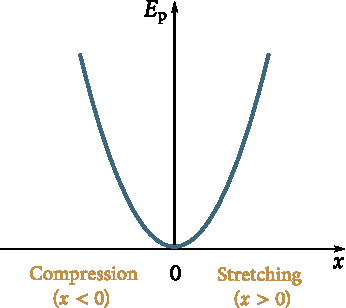
\includegraphics[scale=1]{figures/fig_3_13.pdf}
		\caption[]{}
		\label{fig:3_13}
	\end{center}
	\vspace{-0.7cm}
\end{figure}

The work determined by \eqn{3_14} is done in the elastic longitudinal deformation of a bar or rod. Accordingly, the potential energy of an elastically deformed rod is
\begin{equation}\label{eq:3_79}
E_{\text{p}} = \frac{E\varepsilon^2}{2}\,V
\end{equation}

\noindent
where $E$ is the Young's modulus, $\varepsilon$ is the relative elongation and $V$ is the volume of the rod.

Let us introduce the concept of the density of the energy of elastic deformation $w_{\text{e}}$, which we shall define as the ratio of the energy $\deriv{E_{\text{p}}}$ to the volume $\deriv{V}$ in which it is confined:
\begin{equation}\label{eq:3_80}
w_{\text{e}} = \diff{E_{\text{p}}}{V}.
\end{equation}

\noindent
Since the rod is assumed to be homogeneous and its deformation is uniform, \ie, identical at different points of the rod, the energy \eqn{3_79} is also distributed uniformly in the rod. We can therefore consider that
\begin{equation}\label{eq:3_81}
w_{\text{e}} = \frac{E_{\text{p}}}{V} = \frac{E\varepsilon^2}{2}.
\end{equation}

\noindent
This expression also gives the density of the energy of elastic deformation in stretching (or compression) when the deformation is not uniform. In the latter case to find the energy density at a certain point of a rod, the value of $\varepsilon$ at this point must be introduced into \eqn{3_81}.

On the basis of Eqs.~\eqref{eq:2_32}-\eqref{eq:2_34}, it is not difficult to obtain the following equation for the density of the energy of elastic deformation in shear:
\begin{equation}\label{eq:3_82}
w_{\text{e}} = \frac{G\,\gamma^2}{2}
\end{equation}

\noindent
where $G$ is the shear modulus and $\gamma$ is the relative shear.

\section{Equilibrium Conditions of a Mechanical System}\label{sec:3_9}

Let us consider a point particle whose motion is restricted so that it has only one degree of freedom\footnote{By the number of degrees of freedom of a mechanical system is meant the number of independent quantities with whose aid the position of the system can be set. This will be treated in greater detail in Sec.~\ref{sec:11_5}.}. This signifies that its position can be determined with the aid of a single quantity, for example the coordinate $x$. We can take as an example a ball sliding without friction along a stationary wire bent in a vertical plane (\fig{3_14}a).

Another example is a ball attached to the end of a spring and sliding without friction along a horizontal guide wire ( \fig{3_15}a). The ball is acted upon in each case by a conservative force: the force of gravity and the elastic force of the deformed spring, respectively. Plots of the potential energy $E_{\text{p}}$ against $x$ are shown in Figs.~\ref{fig:3_14}b and \ref{fig:3_15}b.

Since the balls move along the relevant wires without friction, the force with which the wire acts on the ball in each case is at right angles to the velocity of the ball and, consequently, does no work on the ball. Therefore, the energy is conserved
\begin{equation}\label{eq:3_83}
E = E_{\text{k}} + E_{\text{p}} = \text{constant}.
\end{equation}

\noindent
It follows from \eqn{3_83} that the kinetic energy can grow only at the expense of a reduction in the potential energy. Hence, if a ball is in a state such that its velocity equals zero and its potential energy is minimum, it will be unable to start moving without external action on it, \ie, it will be in equilibrium.

Values of $x$ equal to $x_0$ correspond to minima of $E_{\text{p}}$ in the graphs (in \fig{3_15}, $x_0$ is the length of the undeformed spring). The condition of a minimum of the potential energy has the form
\begin{equation}\label{eq:3_84}
\diff{E_{\text{p}}}{x} = 0.
\end{equation}

\noindent
In accordance with \eqn{3_32}, the condition~\eqref{eq:3_84} is equivalent to the fact that
\begin{equation}\label{eq:3_85}
F_x = 0
\end{equation}

\noindent
(when $E_{\text{p}}$ is a function of only one variable, we have $\diffinpartial{E_{\text{p}}}{x}=\diffin{E_{\text{p}}}{x}$). Thus, the position corresponding to a minimum of the potential energy has the property that the force acting on the body equals zero.

\begin{figure}[t]
	\begin{minipage}[t]{0.5\linewidth}
		\begin{center}
			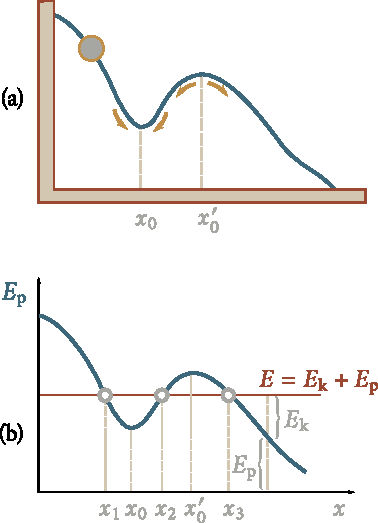
\includegraphics[scale=0.95]{figures/fig_3_14.pdf}
			\caption[]{}
			\label{fig:3_14}
		\end{center}
	\end{minipage}
	\hspace{-0.05cm}
	\begin{minipage}[t]{0.5\linewidth}
		\begin{center}
			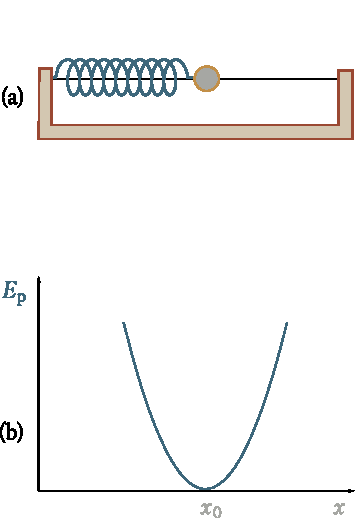
\includegraphics[scale=0.95]{figures/fig_3_15.pdf}
			\caption[]{}
			\label{fig:3_15}
		\end{center}
	\end{minipage}
	\vspace{-0.5cm}
\end{figure}

In the case shown in \fig{3_14}, the conditions~\eqref{eq:3_84} and \eqref{eq:3_85} are also observed for $x$ equal to $x_0$ (\ie, for a maximum $E_{\text{p}}$). The position of the ball determined by this value of $x$ will also be an equilibrium one. This equilibrium, however, unlike that at $x=x_0$, will be unstable: it is sufficient to slightly move the ball out of this position, and a force will appear that will move it away from the position $x_0$. The forces appearing when the ball is displaced from its position of stable equilibrium (for which $x=x_0$) are directed so that they tend to return the ball to its equilibrium position.

Knowing the form of the function expressing the potential energy, we can arrive at a number of conclusions on the nature of motion of a particle. We shall explain this using the graph shown in \fig{3_14}b to describe the motion of our particle. If the total energy has the value shown in the figure, then the particle can move either within the limits from $x_1$ to $x_2$, or within the limits from $x_3$ to infinity. The particle cannot penetrate into the regions with $x<x_1$ and $x_2<x<x_3$ because its potential energy cannot become greater than its total energy (if this occurred, then the kinetic energy would be negative). Thus, the region $x_2<x<x_3$ is a \textbf{potential barrier through} which the particle cannot penetrate having its given stock of total energy. The region $x_1<x<x_2$ is called a \textbf{potential well}.

If a particle in its motion cannot move away to infinity, the motion is called \textbf{finite}. If the particle can travel any distance away, the motion is called \textbf{infinite}. A particle in a potential well performs finite motion. The motion of a particle with a negative total energy in the central field of forces of attraction will also be finite (it is assumed that the potential energy vanishes at infinity).

\section{Law of Momentum Conservation}\label{sec:3_10}

In the preceding sections, we considered the additive integral of motion called energy. Let us find another additive quantity that is conserved for a closed system. For this purpose, we shall consider a system of $N$ interacting particles. Assume that external forces whose resultant is $\vec{F}_i$ act on the $i$-th particle in addition to the internal forces $\vec{F}_{ik}$. Let us write \eqn{2_10} for all the $N$ particles:
\begin{align*}
\dot{\vec{p}}_1 &= \vec{F}_{12} + \vec{F}_{13} + \ldots + \vec{F}_{1k} + \ldots + \vec{F}_{1N} + \vec{F}_{1} = \sum_{k=2}^{N} \vec{F}_{1k} + \vec{F}_{1}\\
\dot{\vec{p}}_2 &= \vec{F}_{21} + \vec{F}_{23} + \ldots + \vec{F}_{2k} + \ldots + \vec{F}_{2N} + \vec{F}_{2} = \sum_{\substack{k=1\\(k\neq 2)}}^{N} \vec{F}_{2k} + \vec{F}_{2}\\
&\cdots \quad\quad\quad\cdots \quad\quad\quad\cdots \quad\quad\quad\cdots \quad\quad\quad\cdots\\
\dot{\vec{p}}_i &= \vec{F}_{i1} + \vec{F}_{i2} + \ldots + \vec{F}_{ik} + \ldots + \vec{F}_{iN} + \vec{F}_{i} = \sum_{\substack{k=1\\(k\neq i)}}^{N} \vec{F}_{ik} + \vec{F}_{i}\\
&\cdots \quad\quad\quad\cdots \quad\quad\quad\cdots \quad\quad\quad\cdots \quad\quad\quad\cdots\\
\dot{\vec{p}}_N &= \vec{F}_{N1} + \vec{F}_{N2} + \ldots + \vec{F}_{Nk} + \ldots + \vec{F}_{N,N-1} + \vec{F}_{N} = \sum_{k=1}^{N-1} \vec{F}_{Nk} + \vec{F}_{N}
\end{align*}

Let us find the sum of these $N$ equations. Since $\vec{F}_{12}+\vec{F}_{21}=0$, etc., only the external forces will remain in the right-hand side. We thus arrive at the relation
\begin{equation}\label{eq:3_86}
\frac{\upd}{\deriv{t}}(\vec{p}_1+\vec{p}_2+\ldots+\vec{p}_N) = \vec{F}_1+\vec{F}_2+\ldots+\vec{F}_N = \sum_{i=1}^{N} \vec{F}_i
\end{equation}

The sum of the momenta of the particles forming a mechanical system is called the \textbf{momentum of the system}. Denoting this momentum by $\vec{p}$, we find that
\begin{equation}\label{eq:3_87}
\vec{p} = \sum_{i=1}^{N} \vec{p}_i = \sum_{i=1}^{N} m_i\vec{v}_i.
\end{equation}

\noindent
It follows from \eqn{3_87} that the momentum is an additive quantity.

Let us write \eqn{3_86} in the form
\begin{equation}\label{eq:3_88}
\diff{\vec{p}}{t} = \sum_{i=1}^{N} \vec{F}_i.
\end{equation}

\noindent
Hence it follows that in the absence of external forces, $\diffin{\vec{p}}{t}=0$. Consequently, for a closed system, $\vec{p}$ is constant. This statement forms the content of the \textbf{law of momentum conservation}, which is formulated as follows: \textit{the momentum of a closed system of point particles remains constant}.

It should be noted that the momentum also remains constant for an unclosed system provided that the sum of the external forces is zero [see \eqn{3_88}]. When the sum of the external forces does not equal zero, but the projection of this sum on a certain direction does equal zero, the component of the momentum in this direction is conserved. Indeed, upon projecting all the quantities of \eqn{3_88} onto a certain direction $x$, we find that
\begin{equation}\label{eq:3_89}
\diff{p_x}{t} = \sum_{i=1}^{N} F_{xi}
\end{equation}

\noindent
whence our statement follows. [We remind our reader that $(\diffin{\vec{p}}{t})_{\text{pr. }\vec{x}}=\diffin{p_x}{t}$, see Eqs.~\eqref{eq:1_40}].

The momentum of a system of particles can be represented as the product of the total mass of the particles and the velocity of the centre of mass of the system:
\begin{equation}\label{eq:3_90}
\vec{p} = m\vec{v}_{\text{C}}
\end{equation}

The \textbf{centre of mass} (or the \textbf{centre of inertia}) of a system is defined as the point C whose position is set by the position vector $\vec{r}_{\text{C}}$ determined as follows:
\begin{equation}\label{eq:3_91}
\vec{r}_{\text{C}} = \frac{m_1\vec{r}_1+m_2\vec{r}_2+\ldots+m_N\vec{r}_N}{m_1+m_2+\ldots+m_N} = \frac{\sum_{i=1}^N m_i\vec{r}_i}{\sum_{i=1}^N m_i} = \frac{1}{m} \sum_{i=1}^N m_i\vec{r}_i
\end{equation}

\noindent
where $m_i$ is the mass of the $i$-th particle, $\vec{r}_i$ the position vector determining the position of this particle, and  $m$ the mass of the system.

The Cartesian coordinates of the centre of mass equal the projections of $\vec{r}_{\text{C}}$ onto the coordinate axes:
\begin{equation}\label{eq:3_92}
x_{\text{C}} = \frac{1}{m} \sum_{i=1}^N m_i x_i,\quad y_{\text{C}} = \frac{1}{m} \sum_{i=1}^N m_i y_i,\quad
z_{\text{C}} = \frac{1}{m} \sum_{i=1}^N m_i z_i.
\end{equation}

\noindent
It must be noted that in a homogeneous field of gravity forces the centre of mass coincides with the centre of gravity of a system.

We find the velocity of the centre of mass by time differentiation of the position vector~\eqref{eq:3_91}:
\begin{equation*}
\vec{v}_{\text{C}} = \dot{\vec{r}}_{\text{C}} = \frac{1}{m}\sum_{i=1}^N m_i\dot{\vec{r}}_i = \frac{1}{m} \sum_{i=1}^N m_i\vec{v}_i = \frac{\vec{p}}{m}
\end{equation*}

\noindent
(see \eqn{3_87}]. Hence follows \eqn{3_90}.

For a closed system, $\vec{p}=m\vec{v}_{\text{C}}=\text{constant}$. Therefore, the centre of mass of a closed system either moves uniformly in a straight line, or remains stationary.

A reference frame in which the centre of mass is at rest is called a \textbf{centre-of-mass} frame or a \textbf{c.m.-frame}. This frame is obviously an inertial one.

A reference frame associated with measuring instruments is called a \textbf{laboratory} or an \textbf{l-frame}.

\section{Collision of Two Bodies}\label{sec:3_11}

When bodies collide with one another, they become deformed.  The kinetic energy which the bodies had before the collision partially or completely transforms into the potential energy of elastic deformation and into the so-called internal energy of the bodies. An increase in the internal energy of bodies is attended by elevation of their temperature.

Two extreme kinds of collisions are distinguished: perfectly elastic and completely inelastic ones. A \textbf{perfectly elastic collision} is one in which the mechanical energy of the bodies does not transform into other non-mechanical kinds of energy. In such a collision, the kinetic energy transforms completely or partly into the potential energy of elastic deformation. Next the bodies return to their original shape, repelling each other. As a result, the potential energy of elastic deformation again transforms into kinetic energy, and the bodies fly apart with velocities whose magnitude and direction are determined by two conditions---conservation of the total energy and conservation of the total momentum of the system of bodies.

A \textbf{completely inelastic collision} is characterized by the fact that no potential energy of deformation is produced. The kinetic energy of the bodies completely or partly transforms into internal energy. After colliding, the bodies either move with the same velocity or are at rest. In a completely inelastic collision, only the law of conservation of momentum is observed. The law of conservation of mechanical energy is not observed---instead of it the law of conservation of the total energy of different kinds-mechanical and internal---is observed.

Let us first consider a completely inelastic collision of two particles (point particles) forming a closed system. Let the masses of the particles be $m_1$ and $m_2$, and their velocities before colliding $\vec{v}_{10}$ and $\vec{v}_{20}$. In view of the law of momentum conservation, the total momentum of the particles after the collision must be the same as before it:
\begin{equation}\label{eq:3_93}
m_1\vec{v}_{10} + m_2\vec{v}_{20} = m_1\vec{v} + m_2\vec{v} = (m_1+m_2) \vec{v}
\end{equation}

\noindent
($\vec{v}$ is the identical velocity of both particles after colliding). It follows from \eqn{3_93} that
\begin{equation}\label{eq:3_94}
\vec{v} = \frac{m_1\vec{v}_{10} + m_2\vec{v}_{20}}{m_1+m_2}. 
\end{equation}

\noindent
For practical calculations, \eqn{3_94} must be projected onto the correspondingly selected directions.


Let us now consider a perfectly elastic collision. We shall limit ourselves to the case of a central collision of two homogeneous spheres. A collision is called central if the spheres before colliding travelled along the straight line passing through their centres. A central collision of two spheres can take place (1) if the spheres are moving toward each other (\fig{3_16}a), or (2) if one of the spheres is overtaking the other one (\fig{3_16}b).

\begin{figure}[t]
	\begin{center}
		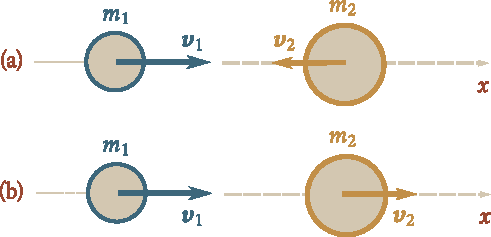
\includegraphics[scale=1]{figures/fig_3_16.pdf}
		\caption[]{}
		\label{fig:3_16}
	\end{center}
	\vspace{-0.7cm}
\end{figure}

We shall assume that the spheres form a closed system or that the external forces applied to them balance each other. We shall also assume that the spheres do not rotate.

Let the masses of the spheres be $m_1$ and $m_2$, the velocities of the spheres before the collision be $\vec{v}_{10}$ and $\vec{v}_{20}$, and, finally, the velocities after the collision be $\vec{v}_{1}$ and $\vec{v}_{2}$. The equations of conservation of energy and momentum are:
\begin{align}
\frac{m_1\vec{v}_{10}^2}{2} + \frac{m_2\vec{v}_{20}^2}{2} &= \frac{m_1\vec{v}_{1}^2}{2} + \frac{m_2\vec{v}_{2}^2}{2}\label{eq:3_95}\\
m_1\vec{v}_{10} + m_2\vec{v}_{20} &= m_1\vec{v}_{1} + m_2\vec{v}_{2}.\label{eq:3_96}
\end{align}

\noindent
Taking into account that $(\vec{a}_2-\vec{b}_2)=(\vec{a}-\vec{b})(\vec{a}+\vec{b})$, we can write \eqn{3_95} in the form
\begin{equation}\label{eq:3_97}
m_1(\vec{v}_{10}-\vec{v}_{1})(\vec{v}_{10}+\vec{v}_{1}) = m_2(\vec{v}_{2}-\vec{v}_{20})(\vec{v}_{2}+\vec{v}_{20}).
\end{equation}

\noindent
Relation \eqn{3_96} can be transformed as follows:
\begin{equation}\label{eq:3_98}
m_1(\vec{v}_{10}-\vec{v}_{1}) = m_2(\vec{v}_{2}-\vec{v}_{20}).
\end{equation}

We can state, from considerations of symmetry, that the velocities of the spheres after the collision will be directed along the same straight line that was the path of the centres of the spheres before colliding. Consequently, all the vectors in Eqs.~\eqref{eq:3_97} and \eqref{eq:3_98} are collinear. For the collinear vectors $\vec{a}, \vec{b}, \vec{c}$, it follows from the equation $\vecdot{a}{b}=\vecdot{a}{c}$ that $\vec{b}=\vec{c}$. Therefore, comparing Eqs.~\eqref{eq:3_97} and \eqref{eq:3_98}, we can conclude that
\begin{equation}\label{eq:3_99}
\vec{v}_{10} + \vec{v}_{1} = \vec{v}_{2} + \vec{v}_{20}.
\end{equation}

\noindent
Multiplying \eqn{3_99} by $m_2$ and subtracting the result from \eqn{3_98}, then multiplying \eqn{3_99} by $m_1$ and adding the result to \eqn{3_98}, we get the velocities of the spheres after the collision:
\begin{equation}\label{eq:3_100}
\vec{v}_1 = \frac{2m_2\vec{v}_{20}+(m_1-m_2)\vec{v}_{10}}{m_1+m_2},\quad \vec{v}_2 = \frac{2m_1\vec{v}_{10}+(m_2-m_1)\vec{v}_{20}}{m_1+m_2}.
\end{equation}

\noindent
For numerical calculations, the relations~\eqref{eq:3_100} must be projected onto the $x$-axis along which the spheres are moving (see \fig{3_16}).

We must note that the velocities of the spheres after a perfectly elastic collision cannot be the same. Indeed, equating expressions~\eqref{eq:3_100} for $\vec{v}_1$ and $\vec{v}_2$ and performing the relevant transformations, we get
\begin{equation*}
\vec{v}_{10} = \vec{v}_{20}.
\end{equation*}

\noindent
Consequently, for the velocities of the spheres to be the same after the collision, they must also be the same before it, but in this case no collision can take place. Hence, it follows that the condition of equality of the velocities of the spheres after the collision is incompatible with the law of conservation of energy.

Let us consider the case when the masses of the colliding spheres are equal: $m_1=m_2$. It follows from Eqs.~\eqref{eq:3_100} that in this condition
\begin{equation*}
\vec{v}_{1} = \vec{v}_{20}\quad \vec{v}_{2} = \vec{v}_{10}
\end{equation*}

\noindent
\ie, the spheres exchange velocities when they collide. Particularly, if one of the spheres of the same mass, for instance, the second one, is stationary before the collision, then after it it will travel with the velocity which the first sphere originally had, while the first sphere after the collision will be stationary.

We can use Eqs.~\eqref{eq:3_100} to find the velocity of a sphere after an elastic collision with a stationary or a moving wall (which we can consider as a sphere of infinitely great mass $m_2$ and infinitely great radius). Dividing the numerator and denominator of Eqs.~\eqref{eq:3_100} by $m_2$ and disregarding the terms containing the factor $m_1/m_2$, we get
\begin{equation*}
\vec{v}_{1} = 2\vec{v}_{20}-\vec{v}_{10}\quad \vec{v}_{2} = \vec{v}_{20}.
\end{equation*}

\noindent
The result obtained shows that the velocity of the wall remains unchanged. The velocity of the sphere, however, if the wall is stationary ($\vec{v}_{20}=0$), reverses. If the wall is moving, the magnitude of the velocity of the sphere also changes (it grows by $2v_{20}$ if the wall moves toward the sphere and diminishes by $2v_{20}$ if the wall moves away from the sphere catching up with it).

\begin{figure}[t]
	\begin{center}
		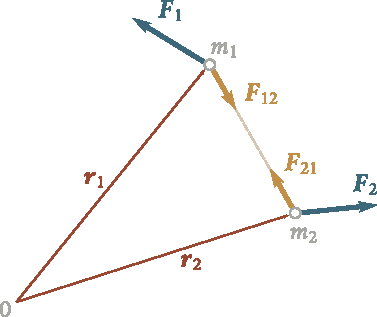
\includegraphics[scale=1]{figures/fig_3_17.pdf}
		\caption[]{}
		\label{fig:3_17}
	\end{center}
	\vspace{-0.7cm}
\end{figure}

\section{Law of Angular Momentum Conservation}\label{sec:3_12}

We already know two additive quantities obeying laws of conservation: energy and momentum. Now we shall find a third quantity of this kind. For this purpose, we shall consider a system consisting of two interacting particles on which external forces also act (\fig{3_17}). The equations of motion of the particles have the form
\begin{equation*}
m_1\dot{\vec{v}}_1 = \vec{F}_{12} + \vec{F}_1,\quad m_2\dot{\vec{v}}_2 = \vec{F}_{21} + \vec{F}_2.
\end{equation*}

\noindent
Let us find the vector product of the first equation and the position vector of the first particle $\vec{r}_1$ and of the second equation and the position vector of the second particle $\vec{r}_2$, placing the position vectors at the left:
\begin{equation}\label{eq:3_101}
\begin{cases}
& \!\!\!\! m_1(\vec{r}_1\times\dot{\vec{v}}_1) = \vecprodind{r}{1}{F}{12} + \vecprodind{r}{1}{F}{1}\\
& \!\!\!\! m_2(\vec{r}_2\times\dot{\vec{v}}_2) = \vecprodind{r}{2}{F}{21} + \vecprodind{r}{2}{F}{2}.
\end{cases}
\end{equation}

A vector product of the kind $\vec{r}\times\dot{\vec{v}}$ is equivalent to the expression $\diffin{(\vec{r}\times\dot{\vec{v}})}{t}$. Indeed, according to \eqn{1_55}
\begin{equation}\label{eq:3_102}
\frac{\upd}{\deriv{t}}(\vec{r}\times\dot{\vec{v}}) = \vec{r}\times\dot{\vec{v}} + \dot{\vec{r}}\times\vec{v} = \vec{r}\times\dot{\vec{v}}
\end{equation}

\noindent
because $\dot{\vec{r}}\times\vec{v}=\vec{v}\times\vec{v}=0$. Making such a substitution in Eqs.~\eqref{eq:3_101} and taking into account that $\vec{F}_{21}=-\vec{F}_{12}$, we get the equations
\begin{equation}\label{eq:3_103}
\begin{cases}
& \!\!\!\! m_1\,\dfrac{\upd}{\deriv{t}}(\vec{r}_1\times\vec{v}_1) = \vecprodind{r}{1}{F}{12} + \vecprodind{r}{1}{F}{1}\\[10pt]
& \!\!\!\! m_2\,\dfrac{\upd}{\deriv{t}}(\vec{r}_2\times\vec{v}_2) = - \vecprodind{r}{2}{F}{12} + \vecprodind{r}{2}{F}{2}.
\end{cases}
\end{equation}

Mass is a constant scalar quantity. It can therefore be put inside the time derivative and into the vector product:
\begin{equation*}
m\,\frac{\upd}{\deriv{t}}(\vec{r}\times\vec{v}) = \frac{\upd}{\deriv{t}}(\vec{r}\times m\vec{v}) = \frac{\upd}{\deriv{t}}(\vec{r}\times\vec{p}).
\end{equation*}

\noindent
With this in view, we shall find the sum of Eqs.~\eqref{eq:3_103}. We get
\begin{equation*}
\frac{\upd}{\deriv{t}}(\vecprodind{r}{1}{p}{1} + \vecprodind{r}{2}{p}{2}) = (\vec{r}_1-\vec{r}_2)\times\vec{F}_{12} + \vecprodind{r}{1}{F}{1} + \vecprodind{r}{2}{F}{2}.
\end{equation*}

\noindent
The vectors $\vec{r}_1-\vec{r}_2$ and $\vec{F}_{12}$ are collinear. Consequently, their vector product equals zero. We thus obtain the relation
\begin{equation}\label{eq:3_104}
\frac{\upd}{\deriv{t}}(\vecprodind{r}{1}{p}{1} + \vecprodind{r}{2}{p}{2}) = \vecprodind{r}{1}{F}{1} + \vecprodind{r}{2}{F}{2}.
\end{equation}

\noindent
If the system is closed, the right-hand side of this relation vanishes, and, therefore,
\begin{equation*}
\vecprodind{r}{1}{p}{1} + \vecprodind{r}{2}{p}{2} = \text{constant}.
\end{equation*}

\noindent
We have arrived at an additive quantity obeying a law of conservation that is called the angular momentum (or the moment of momentum) relative to point $0$ (see \fig{3_17}).

For a separate particle, the angular momentum relative to point $0$ is defined as the pseudovector
\begin{equation}\label{eq:3_105}
\vec{L} = \vecprod{r}{p} = \vec{r}\times m\vec{v}.
\end{equation}

\noindent
The angular momentum of a system relative to point $0$ is defined as the vector sum of the angular momenta of the particles in the system:
\begin{equation}\label{eq:3_106}
\vec{L} = \sum_{i}\vec{L}_i = \sum_{i} \vecprodind{r}{i}{p}{i}.
\end{equation}

The projection of the vector~\eqref{eq:3_105} onto the $z$-axis is called the \textbf{angular momentum of a particle relative to this axis}:
\begin{equation}\label{eq:3_107}
L_z = (\vecprod{r}{p})_{\text{pr.},\vec{z}}.
\end{equation}

\noindent
Similarly, the \textbf{angular momentum of a system relative to the $z$-axis} is defined as the scalar quantity
\begin{equation}\label{eq:3_108}
L_z = \sum_i (\vecprodind{r}{i}{p}{i})_{\text{pr.},\vec{z}}.
\end{equation}

%\begin{figure}[t]
%	\begin{center}
%		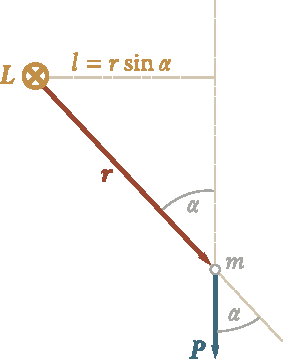
\includegraphics[scale=1]{figures/fig_3_18.pdf}
%		\caption[]{}
%		\label{fig:3_18}
%	\end{center}
%	%	\vspace{-0.7cm}
%\end{figure}

\noindent
A glance at \fig{3_18} shows that the magnitude of the angular momentum vector of a particle is
\begin{equation}\label{eq:3_109}
L = rp\sin\alpha = lp
\end{equation}

\noindent
where $l=r\sin\alpha$ is the length of a perpendicular dropped from point $0$ onto the straight line along which the momentum of the particle is directed. This length is called the arm of the momentum relative to point $0$. It is assumed in \fig{3_18} that point $0$ relative to which the angular momentum is taken and the vector $\vec{p}$ are in the plane of the drawing. The vector $\vec{L}$ is at right angles to the plane of the drawing and is directed away from us.

Let us consider two typical examples.
\begin{enumerate}[1.]
	\item Assume that a particle is moving along the straight line depicted in \fig{3_18} by the dash line. In this case, the angular momentum 	of the particle can change only in magnitude. The magnitude of the angular momentum is
	\begin{equation}\label{eq:3_110}
	L = mvl
	\end{equation}
	
	\noindent
	the arm $l$ remaining constant here.
	\item A particle of mass $m$ moves along a circle of radius $R$ (\fig{3_19}). The magnitude of the angular momentum of the particle relative to the centre of the circle $0$ is
	\begin{equation}\label{eq:3_111}
	L = mvR
	\end{equation}
	
	\noindent
	The vector $\vec{L}$ is perpendicular to the plane of the circle. The direction of motion of the particle and the vector $\vec{L}$ form a right-handed system. Since the arm, which equals $R$, remains constant, the angular momentum can change only as a result of a change in the magnitude of the velocity. Upon uniform motion of the particle along the circle, the angular momentum remains constant both in magnitude and in direction.
\end{enumerate}

\begin{figure}[t]
	\begin{minipage}[t]{0.5\linewidth}
		\begin{center}
			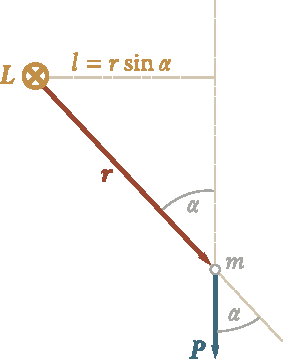
\includegraphics[scale=0.95]{figures/fig_3_18.pdf}
			\caption[]{}
			\label{fig:3_18}
		\end{center}
	\end{minipage}
	\hspace{-0.05cm}
	\begin{minipage}[t]{0.5\linewidth}
		\begin{center}
			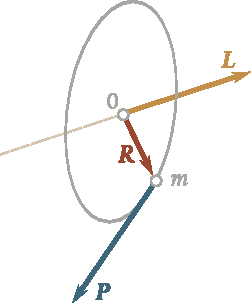
\includegraphics[scale=0.95]{figures/fig_3_19.pdf}
			\caption[]{}
			\label{fig:3_19}
		\end{center}
	\end{minipage}
	\vspace{-0.3cm}
\end{figure}

The pseudovector
\begin{equation}\label{eq:3_112}
\vec{M} = \vecprod{r}{F}
\end{equation}

\noindent
is called the moment of the force $\vec{F}$ relative to point $0$ (or the torque relative to this point) from which the position vector $\vec{r}$ is drawn to the point of application of the force (\fig{3_20}). Inspection of the figure shows that the magnitude of the moment of the force can be written in the form
\begin{equation}\label{eq:3_113}
M = rF\sin\alpha = lF
\end{equation}

\noindent
where $l=r\sin\alpha$ is the arm of the force (the moment or lever arm) relative to point $0$ (\ie, the length of a perpendicular dropped from point $0$ onto the straight line along which the force acts).

The projection of the vector $\vec{M}$ onto an axis $z$ passing through point $0$ relative to which $\vec{M}$ has been determined is called the moment of the force (the torque) relative to this axis:
\begin{equation}\label{eq:3_114}
M_z = \vecprod{r}{F}_{\text{pr.},\vec{z}}.
\end{equation}

\begin{figure}[t]
	\begin{minipage}[t]{0.5\linewidth}
		\begin{center}
			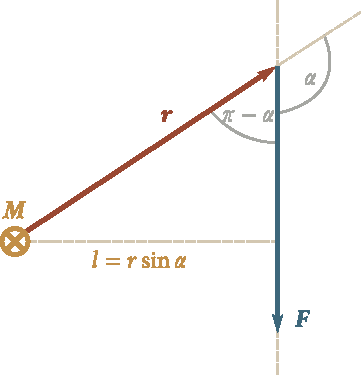
\includegraphics[scale=0.9]{figures/fig_3_20.pdf}
			\caption[]{}
			\label{fig:3_20}
		\end{center}
	\end{minipage}
	\hspace{-0.05cm}
	\begin{minipage}[t]{0.5\linewidth}
		\begin{center}
			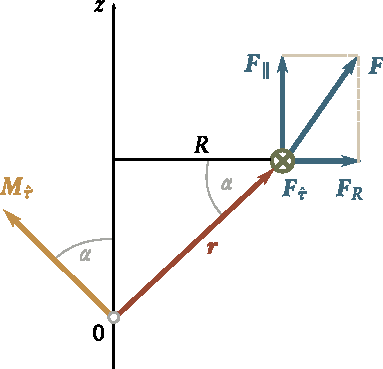
\includegraphics[scale=0.9]{figures/fig_3_21.pdf}
			\caption[]{}
			\label{fig:3_21}
		\end{center}
	\end{minipage}
	\vspace{-0.3cm}
\end{figure}

\noindent
Let us resolve the force vector $\vec{F}$ (\fig{3_21}) into three mutually perpendicular components: $\vec{F}_{\parallel}$ parallel to the $z$-axis, $\vec{F}_R$ perpendicular to the $z$-axis and acting along a line passing through the axis, and, finally, $\vec{F}_{\hatvec{\tau}}$ perpendicular to the plane passing through the axis and the point of application of the force (this component is designated in the figure by a circle with a cross in it). If we imagine a circle of radius $R$ with its centre on the $z$-axis, then the component $\vec{F}_{\hatvec{\tau}}$ will be directed along a tangent to this circle. The moment of the force $\vec{F}$ relative to point $0$ equals the sum of the moments of the components: $\vec{M}=\vec{M}_{\parallel}+\vec{M}_R+\vec{M}_{\hatvec{\tau}}$. The vectors $\vec{M}_{\parallel}$, and $\vec{M}_R$ are perpendicular to the $z$-axis, therefore their projections onto this axis equal zero. The moment $\vec{M}_{\hatvec{\tau}}$ has a magnitude equal to $rF_{\hatvec{\tau}}$ and makes the angle $\alpha$ with the $z$-axis. The cosine of $\alpha$ is $R/r$. Hence, the moment of the component $\vec{F}_{\hatvec{\tau}}$ relative to the $z$-axis has the magnitude $\vec{M}_{\hatvec{\tau}}\cos\alpha=RF_{\hatvec{\tau}}$. The moment of the force $\vec{F}$ relative to the $z$-axis thus equals
\begin{equation}\label{eq:3_115}
M_z = RF_{\hatvec{\tau}}.
\end{equation}

\noindent
Up to now, we understood $F_{\hatvec{\tau}}$ to stand for the magnitude of the component $\vec{F}_{\hatvec{\tau}}$. But $F_{\hatvec{\tau}}$ can also be considered as the projection of the vector $\vec{F}$ onto the unit vector $\hatvec{\tau}$ that is tangent to a circle of radius $R$ and is directed so that motion along the circle in the direction of $\hatvec{\tau}$ forms a right-handed system with the direction of the $z$-axis. With such an interpretation of $F_{\hatvec{\tau}}$, \eqn{3_115} will also determine the sign of $M_z$.

The moment $\vec{M}$ of a force characterizes the ability of the force to rotate a body about the point relative to which it is taken. We must note that when a body can rotate arbitrarily relative to point $0$, the force will cause it to rotate about an axis that is perpendicular to the plane containing the force and point $0$, \ie, about an axis coinciding with the direction of the moment of the force relative to the given point.

The moment of a force relative to the $z$-axis characterizes the ability of the force to rotate a body about this axis. The components $\vec{F}_{\parallel}$ and $\vec{F}_{R}$ cannot cause rotation about the $z$-axis. Such rotation can be produced only by the component $\vec{F}_{\hatvec{\tau}}$, and the success of the rotation will grow with an increasing moment arm $R$.

\begin{figure}[t]
	\begin{center}
		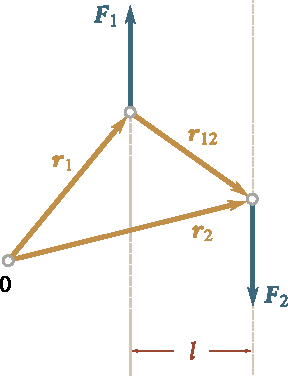
\includegraphics[scale=0.94]{figures/fig_3_22.pdf}
		\caption[]{}
		\label{fig:3_22}
	\end{center}
	\vspace{-0.75cm}
\end{figure}

Two equal, parallel and oppositely directed forces are called \textbf{a force couple} (\fig{3_22}). The distance $l$ between the lines along which the forces act is called the arm of the couple. The total moment of the forces $\vec{F}_1$ and $\vec{F}_2$ forming the couple is
\begin{equation*}
\vec{M} = \vecprodind{r}{1}{F}{1} + \vecprodind{r}{2}{F}{2}.
\end{equation*}

\noindent
Since $\vec{F}_1=-\vec{F}_2$, we can write
\begin{equation}\label{eq:3_116}
\vec{M} = -\vecprodind{r}{1}{F}{2} + \vecprodind{r}{2}{F}{2} = (\vec{r}_2 - \vec{r}_1)\times\vec{F}_2 = \vecprodind{r}{12}{F}{2}
\end{equation}

\noindent
where $\vec{r}_{12}=\vec{r}_2-\vec{r}_1$ is the vector drawn from the point of application of the force $\vec{F}_1$ to the point of application of $\vec{F}_2$. Equation~\eqref{eq:3_116} does not depend on the choice of point $0$. Consequently, the moment of a force couple relative to any point will be the same. The vector of the moment of a force couple is perpendicular to the plane containing the forces (see \fig{3_22}) and numerically equals the product of the magnitude of any of the forces and the arm.

%\begin{figure}[t]
%	\begin{minipage}[t]{0.5\linewidth}
%		\begin{center}
%			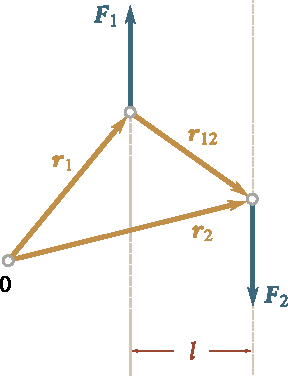
\includegraphics[scale=0.95]{figures/fig_3_22.pdf}
%			\caption[]{}
%			\label{fig:3_22}
%		\end{center}
%	\end{minipage}
%	\hspace{-0.05cm}
%	\begin{minipage}[t]{0.5\linewidth}
%		\begin{center}
%			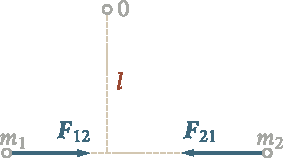
\includegraphics[scale=0.95]{figures/fig_3_23.pdf}
%			\caption[]{}
%			\label{fig:3_23}
%		\end{center}
%	\end{minipage}
%	\vspace{-0.3cm}
%\end{figure}

Forces of interaction between particles act in opposite directions along the same straight line (\fig{3_23}). Their moments relative to an arbitrary point $0$ are equal in magnitude and opposite in direction. Therefore, the moments of the internal forces balance one another in pairs, and the sum of the moments of all the internal forces for any system of particles, particularly for a solid body, always equals zero:
\begin{equation}\label{eq:3_117}
\sum\vec{M}_{\text{int}} = 0.
\end{equation}

In accordance with definitions~\eqref{eq:3_106} and~\eqref{eq:3_112}, we can write \eqn{3_104} as follows:
\begin{equation}\label{eq:3_118}
\frac{\upd}{\deriv{t}}\vec{L} = \sum\vec{M}_{\text{ext}}.
\end{equation}

\noindent
This equation is similar to \eqn{3_88}. A comparison of these equations shows that just like the time derivative of the momentum of a system equals the sum of the external forces, so does the time derivative of the angular momentum equal the sum of the moments of the external forces.

\begin{figure}[t]
	\begin{center}
		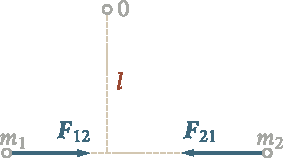
\includegraphics[scale=0.9]{figures/fig_3_23.pdf}
		\caption[]{}
		\label{fig:3_23}
	\end{center}
	\vspace{-0.9cm}
\end{figure}

It follows from \eqn{3_118} that in the absence of external forces $\diffin{\vec{L}}{t}$. Hence, $\vec{L}$ is constant for a closed system. This statement is the content of the \textbf{law of angular momentum conservation}, which is formulated as follows: \textit{the angular momentum of a closed system of point particles remains constant}.

We have proved \eqn{3_118} for a system of two particles. It can be generalized quite simply, however, for any number of particles. Let us write the equations of motion of the particles:
\begin{align*}
m_1\dot{\vec{v}}_1 &= \sum_k \vec{F}_{1k} + \vec{F}_1\\
\cdots & \quad\cdots \quad\cdots\\
m_i\dot{\vec{v}}_i &= \sum_k \vec{F}_{ik} + \vec{F}_i\\
\cdots & \quad\cdots \quad\cdots\\
m_N\dot{\vec{v}}_N &= \sum_k \vec{F}_{Nk} + \vec{F}_N
\end{align*}

\noindent
Multiplying each of the equations by the corresponding position vector, we get [see \eqn{3_102}]:
\begin{align*}
\frac{\upd}{\deriv{t}}(\vecprodind{r}{1}{p}{1}) &= \sum_k \vecprodind{r}{1}{F}{1k} + \vecprodind{r}{1}{F}{1}\\
\cdots\quad\quad\cdots & \quad\quad\cdots \quad\quad\cdots \quad\quad\cdots\\
\frac{\upd}{\deriv{t}}(\vecprodind{r}{i}{p}{i}) &= \sum_k \vecprodind{r}{i}{F}{ik} + \vecprodind{r}{i}{F}{i}\\
\cdots\quad\quad\cdots & \quad\quad\cdots \quad\quad\cdots \quad\quad\cdots\\
\frac{\upd}{\deriv{t}}(\vecprodind{r}{N}{p}{N}) &= \sum_k \vecprodind{r}{N}{F}{Nk} + \vecprodind{r}{N}{F}{N}.
\end{align*}

\noindent
Let us add up all the $N$ equations:
\begin{equation*}
\frac{\upd}{\deriv{t}} \sum_i \vec{L}_i = \sum_{\substack{i=k\\(i\neq k)}} \vecprodind{r}{i}{F}{ik} + \vecprodind{r}{i}{F}{i}.
\end{equation*}

\noindent
The first sum in the right-hand side is the sum of the moments of all the internal forces, which, as we have shown, equals zero [see \eqn{3_117}]. The second sum in the right-hand side is the sum of the moments of the external forces. Consequently, we have arrived at \eqn{3_118}.

We must note that the angular momentum also remains constant for an unclosed system provided that the total moment of the external forces equals zero [see \eqn{3_118}].

Projection of all the quantities in \eqn{3_118} onto a certain direction $z$ yields
\begin{equation}\label{eq:3_119}
\frac{\upd}{\deriv{t}} L_z = \sum M_{z,\text{ext}}
\end{equation}

\noindent
according to which the time derivative of the angular momentum of the system relative to the $z$-axis equals the sum of the moments of the external forces relative to this axis.

It follows from \eqn{3_119} that when the sum of the moments of the external forces relative to an axis equals zero, the angular momentum of the system relative to this axis remains constant.

\section{Motion in a Central Force Field}\label{sec:3_13}

Let us consider a particle in a central force field. We remind our reader that the direction of the force acting on a particle at any point of such a field passes through point $0$---the centre of the field---while the magnitude of the force depends only on the distance from this centre. It is easy to see that the dependence of the force $\vec{F}$ on $\vec{r}$ has the form
\begin{equation}\label{eq:3_120}
\vec{F} = f(r) \vecuni{r}
\end{equation}

\noindent
where $\vecuni{r}$ is the unit vector of the position vector (\fig{3_24}), and $f(r)$ is the projection of the force vector onto the direction of the position vector, \ie, $F_r$. The function $f(r)$ is positive for a repulsive force, and negative for an attractive one. Figure~\ref{fig:3_24} has been drawn for the case of repulsion of a particle from the force centre. Equation~\eqref{eq:3_120} naturally holds only if the origin of coordinates (\ie, the point from which the position vectors are drawn) is at the centre of the field.

\begin{figure}[t]
	\hspace{-0.5cm}
	\begin{minipage}[t]{0.5\linewidth}
		\begin{center}
			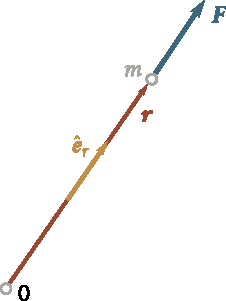
\includegraphics[scale=0.9]{figures/fig_3_24.pdf}
			\caption[]{}
			\label{fig:3_24}
		\end{center}
	\end{minipage}
	\hspace{-0.5cm}
	\begin{minipage}[t]{0.5\linewidth}
		\begin{center}
			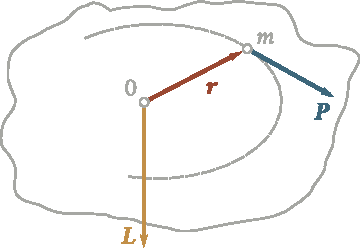
\includegraphics[scale=0.95]{figures/fig_3_25.pdf}
			\caption[]{}
			\label{fig:3_25}
		\end{center}
	\end{minipage}
	\vspace{-0.3cm}
\end{figure}

The moment of the force~\eqref{eq:3_120} relative to point $0$ obviously equals zero. This follows from the fact that the moment arm equals zero. Hence, in accordance with \eqn{3_118}, we see that the angular momentum of a particle moving in a central force field remains constant. The vector $\vec{L}=\vecprod{r}{p}$ at each moment of time is perpendicular to the plane formed by the vectors $\vec{r}$ and $\vec{p}$ (\fig{3_25}). If $\vec{L}=\text{constant}$, this plane will be fixed. Thus, when a particle moves in a central force field, its position vector always remains in one plane. The vector $\vec{p}$ is also permanently in the same plane. Consequently, the trajectory of the particle is a plane curve. The plane containing the trajectory passes through the centre of the field (see \fig{3_25}).

Figure~\ref{fig:3_26} shows a portion of the trajectory of the particle (the vector $\vec{L}$ is directed beyond the drawing). During the time $\deriv{t}$, the position vector of the particle describes the shaded area $\deriv{S}$. This area equals half the area of the parallelogram constructed on the vectors $\vec{r}$ and $\vec{v}\,\deriv{t}$. The area of the parallelogram, in turn, equals the magnitude of the vector product $\vec{r}\times\vec{v}\,\deriv{t}$ [see the text following \eqn{1_28}]. Thus, the area of the shaded triangle is
\begin{equation*}
\deriv{S} = \frac{1}{2}|\vecprod{r}{v}|\,\deriv{t} = \frac{1}{2m}|\vecprod{r}{p}|\,\deriv{t} = \frac{1}{2m}L\,\deriv{t}
\end{equation*}

\noindent
(we have put the scalar multiplier $\deriv{t}$ outside the symbol of the vector product). Dividing both sides of the equation obtained by $\deriv{t}$, we find that
\begin{equation}\label{eq:3_121}
\diff{S}{t} = \diff{L}{2m}.
\end{equation}

The quantity $\diffin{S}{t}$, \ie, the area described by the position vector of a particle in unit time, is called the \textbf{sector velocity}. In a central force field, $L=\text{constant}$, hence the sector velocity of a particle also remains constant.

Let us find an expression for the angular momentum of a particle in the polar coordinates $r$ and $\varphi$ (\fig{3_27}). According to Eqs.~\eqref{eq:1_68}-\eqref{eq:1_71}, the vector velocity of the particle can he represented in the form
\begin{equation}\label{eq:3_122}
\vec{v} = \vec{v}_r + \vec{\varphi} = \dot{r}\vecuni{r} + r\dot{\varphi}\vecuni{\varphi}.
\end{equation}

\noindent
Using this expression in the equation for $\vec{L}$, we get
\begin{equation*}
\vec{L} = m(\vecprod{r}{v}) = m(\vecprod{r}{v}_r) + m(\vecprod{r}{v}_{\varphi}).
\end{equation*}

\noindent
The vectors $\vec{r}$ and $\vec{v}_r$ are collinear, therefore the first addend equals zero. Consequently
\begin{equation*}
\vec{L} = m(\vecprod{r}{v}_{\varphi}) = m(\vec{r}\times r\dot{\varphi}\vecuni{\varphi}) = mr\dot{\varphi}(\vec{r}\times\vecuni{\varphi}).
\end{equation*}

\noindent
The vector product $\vec{r}\times\vecuni{\varphi}$ equals $r\vecuni{z}$, where $\vecuni{z}$, is the unit vector of the $z$-axis (in \fig{3_27} this unit vector is directed toward us). Thus,
\begin{equation}\label{eq:3_123}
\vec{L} = mr^2\dot{\varphi}\vecuni{z}.
\end{equation}

\begin{figure}[t]
%	\hspace{-0.5cm}
	\begin{minipage}[t]{0.5\linewidth}
		\begin{center}
			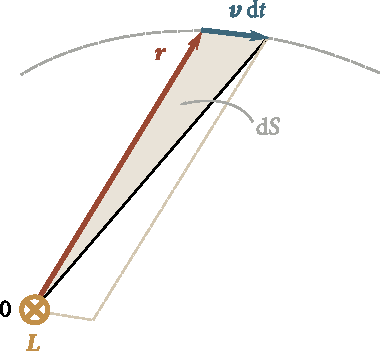
\includegraphics[scale=0.95]{figures/fig_3_26.pdf}
			\caption[]{}
			\label{fig:3_26}
		\end{center}
	\end{minipage}
	\hspace{-0.05cm}
	\begin{minipage}[t]{0.5\linewidth}
		\begin{center}
			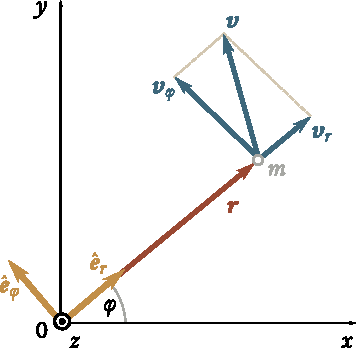
\includegraphics[scale=0.95]{figures/fig_3_27.pdf}
			\caption[]{}
			\label{fig:3_27}
		\end{center}
	\end{minipage}
	\vspace{-0.3cm}
\end{figure}

\noindent
Hence we conclude that
\begin{equation}\label{eq:3_124}
L_z = mr^2\dot{\varphi}
\end{equation}

\noindent
where $L_z$ is the projection of the angular momentum onto the $z$-axis. The magnitude of the angular momentum equals the magnitude of \eqn{3_124}.

Let us now turn to the energy of a particle. Central forces are conservative (see Sec.~\ref{sec:3_4}). According to \eqn{3_30}, the work of a conservative force equals the decrement of the potential energy of the particle $E_{\text{p}}$. Hence, for the force~\eqref{eq:3_120}, the relation $\deriv{A}=-\deriv{E_{\text{p}}}$ holds, \ie,
\begin{equation*}
\deriv{E_{\text{p}}} = -\deriv{A} = f(r)\vecuni{r}\,\deriv{\vec{r}} = -f(r)\,\deriv{r}.
\end{equation*}

\noindent
Integration of this expression yields
\begin{equation}\label{eq:3_125}
E_{\text{p}} = -\int f(r)\,\deriv{r}.
\end{equation}

\noindent
It follows from \eqn{3_125} that the potential energy of a particle in a field of central forces depends only on the distance $r$ from the centre: $E_{\text{p}}=E_{\text{p}}(r)$.

Of special interest are forces inversely proportional to the square of the distance from the force centre. The function $f(r)$ in \eqn{3_120} has the following form for them:
\begin{equation}\label{eq:3_126}
f(r) = \frac{\alpha}{r^2}
\end{equation}

\noindent
where $\alpha$ is a constant quantity ($\alpha>0$ corresponds to repulsion from the centre, and $\alpha<0$ to attraction to the centre). Among such forces are gravitational and Coulomb ones.

Introduction of the function~\eqref{eq:3_126} into \eqn{3_125} yields
\begin{equation*}
E_{\text{p}} = -\alpha \int \frac{\deriv{r}}{r^2} = \frac{\alpha}{r} + C
\end{equation*}

\noindent
where $C$ is an integration constant. The potential energy is conventionally considered to vanish at infinity (\ie, at $r=\infty$). In this condition, $C=0$, and
\begin{equation}\label{eq:3_127}
E_{\text{p}} = \frac{\alpha}{r}.
\end{equation}

\noindent
Thus, the total mechanical energy of a particle moving in a central field of forces that are inversely proportional to the square of the distance from the centre is determined by the expression
\begin{equation}\label{eq:3_128}
E = \frac{mv^2}{2} + \frac{\alpha}{r}.
\end{equation}

\noindent
Substituting the sum of the squares of the velocities $\vec{v}_r$ and $\vec{v}_{\varphi}$, for the square of the velocity $\vec{v}$ in accordance with \eqn{3_122}, \ie, substituting the expression $r^2+r^2\dot{\varphi}^2$ for $v^2$, we obtain
\begin{equation}\label{eq:3_129}
E = \frac{m\dot{r}^2}{2} + \frac{mr^2\dot{\varphi}^2}{2} + \frac{\alpha}{r}.
\end{equation}

The energy and the angular momentum of a particle are conserved in a central field. Consequently, the left-hand sides of Eqs.~\eqref{eq:3_124} and \eqref{eq:3_129} are constants. We have thus arrived at a system of two differential equations:
\begin{equation}\label{eq:3_130}
\begin{cases}
\quad\quad\quad\quad\,\,\,\,\, mr^2\dot{\varphi}^2 \!\!\!\!&= L_z = \text{constant}\\
m\dot{r}^2 + mr^2\dot{\varphi}^2 + \dfrac{2\alpha}{r} \!\!\!\!&= 2E = \text{constant}.
\end{cases}
\end{equation}

\noindent
After integrating these equations, we can find $r$ and $\varphi0$ as functions of $t$, \ie, the trajectory and the nature of motion of the particle. It must be noted that Eqs.~\eqref{eq:3_130} contain the first time derivatives of $r$ and $\varphi$. They are, therefore, much easier to solve than equations following from Newton's laws, which contain the second derivatives of the coordinates.

\begin{figure}[t]
	%	\hspace{-0.5cm}
	\begin{minipage}[t]{0.5\linewidth}
		\begin{center}
			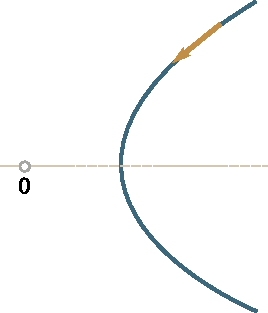
\includegraphics[scale=1]{figures/fig_3_28.pdf}
			\caption[]{}
			\label{fig:3_28}
		\end{center}
	\end{minipage}
	\hspace{-0.2cm}
	\begin{minipage}[t]{0.5\linewidth}
		\begin{center}
			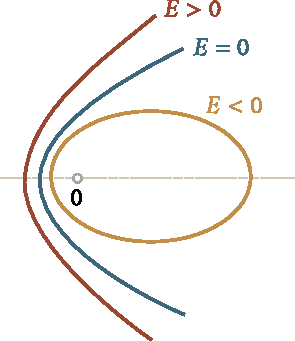
\includegraphics[scale=1]{figures/fig_3_29.pdf}
			\caption[]{}
			\label{fig:3_29}
		\end{center}
	\end{minipage}
	\vspace{-0.3cm}
\end{figure}

Solution of the system of equations~\eqref{eq:3_130} is beyond the scope of this book. We shall limit ourselves to giving the final result. The trajectory of the particle is a conical section, \ie, an ellipse, or a parabola, or a hyperbola. Which of these curves is observed in a given concrete case depends on the sign of the constant $\alpha$ and the magnitude of the total energy of the particle.

For repulsion (\ie, when $\alpha>0$), the trajectory of the particle can only be a hyperbola (\fig{3_28}). If $L_z=0$, the hyperbola degenerates into a straight line whose continuation passes through the force centre. We must note that when $\alpha>0$, the total energy~\eqref{eq:3_128} cannot be negative.

For attraction (\ie, when $alpha<0$), the total energy may be either positive or negative; in particular, it may equal zero. When $E>0$, the trajectory is a hyperbola (\fig{3_29}). When $E=0$, the trajectory will be a parabola. This case takes place if a particle begins its motion from a state of rest at infinity (see \eqn{3_128}]. Finally, when $E<0$, the trajectory will be an ellipse. At values of the energy and the angular momentum complying with the condition that $E=- m\alpha^2/(2L^2)$, the ellipse degenerates into a circle.

Motion along an ellipse is finite, and that along a parabola or hyperbola---infinite (see Sec.~\ref{sec:3_9}).

\section{Two-Body Problem}\label{sec:3_19}

A two-body problem is the name given to a problem on the motion of two interacting particles. The system formed by the particles is assumed to be closed. We learned in Sec.~\ref{sec:3_10} that the centre of mass of a closed system is either at rest or moves uniformly in a straight line. We shall solve the problem in a centre-of-mass frame (a c.m. frame), placing the origin of coordinates at point C. In this case, $r_{\text{C}}=(m_1\vec{r}_1+m_2\vec{r}_2)/(m_1+m_2)=0$, \ie,
\begin{equation}\label{eq:3_131}
m_1\vec{r}_1 = -m_2\vec{r}_2
\end{equation}

\noindent
(\fig{3_30}a). Let us introduce the vector
\begin{equation}\label{eq:3_132}
\vec{r} = \vec{r}_2 - \vec{r}_1
\end{equation}

\noindent
determining the whereabouts of the second particle relative to the first one (\fig{3_30}b). By simultaneously solving Eqs.~\eqref{eq:3_131} and \eqref{eq:3_132}, it is easy to find that
\begin{equation}\label{eq:3_133}
\vec{r}_1 = -\frac{m_2}{m_1+m_2}\vec{r},\quad \vec{r}_2 = \frac{m_1}{m_1+m_2}\vec{r}.
\end{equation}

Similarly to \eqn{3_59}, we can write that $\vec{F}_{12}=-\vec{F}_{21}=f(r)\vecuni{r}$, where $f(r)$ is a function of the distance between the particles. It is positive for forces of attraction (\fig{3_30}c) and negative for forces of repulsion. Let us write the equations of motion of our particles:
\begin{equation*}
m_1\ddot{\vec{r}}_1 = f(r)\vecuni{r},\quad m_2\ddot{\vec{r}}_2 = -f(r)\vecuni{r}
\end{equation*}

\begin{figure}[t]
	\begin{center}
		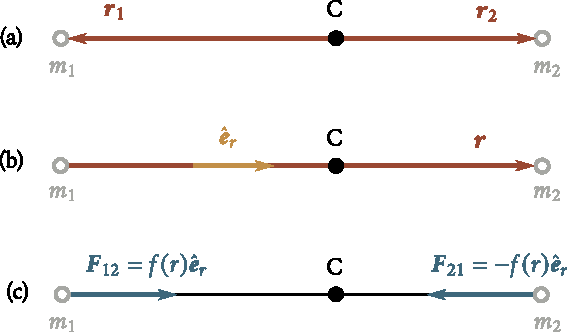
\includegraphics[scale=1]{figures/fig_3_30.pdf}
		\caption[]{}
		\label{fig:3_30}
	\end{center}
\vspace{-0.7cm}
\end{figure}

\noindent
Division of the first equation by $m_1$, of the second one by $m_2$, and subtraction of the first equation from the second yield
\begin{equation*}
\ddot{\vec{r}}_1 - \ddot{\vec{r}}_2 = -\left(\frac{1}{m_1}+\frac{1}{m_2}\right)f(r)\vecuni{r}.
\end{equation*}

\noindent
According to \eqn{3_132}, the left-hand side is $\vec{r}$. Hence,
\begin{equation}\label{eq:3_134}
\ddot{\vec{r}} = -\left(\frac{1}{m_1}+\frac{1}{m_2}\right)f(r)\vecuni{r}.
\end{equation}

\noindent
Equation~\eqref{eq:3_134} can formally be considered as the equation of motion of an imaginary particle in a central force field. The position of the particle relative to the force centre is determined by the position vector $\vec{r}$. According to \eqn{3_134}, the mass $\mu$ determined by the condition that
\begin{equation}\label{eq:3_135}
\frac{1}{\mu} = \frac{1}{m_1} + \frac{1}{m_2}
\end{equation}

\noindent
must be ascribed to our imaginary particle. Hence,
\begin{equation}\label{eq:3_136}
\mu = \frac{m_1m_2}{m_1+m_2}.
\end{equation}

\noindent
The quantity~\eqref{eq:3_136} is called the \textbf{reduced mass} of the particles.

A two-body problem thus consists in a problem on the motion of a single particle in a central force field. Finding $\vec{r}$ as a function of $t$ from \eqn{3_134}, we can use Eqs.~\eqref{eq:3_133} to determine $\vec{r}_1(t)$ and $\vec{r}_2(t)$. The vectors $\vec{r}_1$ and $\vec{r}_2$ are laid off from the centre of mass C of the system. Therefore, to be able to use Eqs.~\eqref{eq:3_133}, we must also lay off the position vector $\vec{r}$ of the imaginary particle from point C [for real particles the vector~\eqref{eq:3_132} is drawn from the first particle to the second one].

It can be seen from Eqs.~\eqref{eq:3_133} and \fig{3_30} that both particles move relative to the centre of mass along geometrically similar trajectories\footnote{When the force of interaction is inversely proportional to the square of the distance between the particles, these trajectories are ellipses, or parabolas, or hyperbolas (see Sec.~\ref{sec:3_13}).}. The straight line joining the particles constantly passes through the centre of mass.

